\appendix
\section{Appendix}
\subsection{Tables}

\begin{table}[!htbp]
    \centering
    \begin{tabular}{|l|r||l|r|}
    \hline
    \textbf{Original Value} & \textbf{Encoded Value} & \textbf{Original Value} & \textbf{Encoded Value} \\
    \hline
    BOWJ & 0 & ILFELEJ & 18 \\
    BROXBRN & 1 & ILFORD & 19 \\
    BRTWOOD & 2 & INGTSTL & 20 \\
    BTHNLGR & 3 & INGTSTN & 21 \\
    CHDWLHT & 4 & IPSWEPJ & 22 \\
    CHESHNT & 5 & IPSWESJ & 23 \\
    CHLMSFD & 6 & IPSWHJN & 24 \\
    CLCHSTR & 7 & IPSWICH & 25 \\
    DISS & 8 & KELVEDN & 26 \\
    FRSTGT & 9 & LIVST & 27 \\
    FRSTGTJ & 10 & MANNGTR & 28 \\
    GIDEAPK & 11 & MANRPK & 29 \\
    GIDEPKJ & 12 & MRKSTEY & 30 \\
    GODMAYS & 13 & MRYLAND & 31 \\
    HAGHLYJ & 14 & NEEDHAM & 32 \\
    HAKNYNM & 15 & NRCH & 33 \\
    HFLPEVL & 16 & NRCHTPJ & 34 \\
    HRLDWOD & 17 & ROMFORD & 35 \\
    SEVNSIS & 36 & STWMDGL & 39 \\
    SHENFLD & 37 & STWMRKT & 40 \\
    STFD & 38 & SVNKNGS & 41 \\
    TROWFLR & 42 & WARE & 45 \\
    TROWSEJ & 43 & WITHAME & 46 \\
    TRWSSBJ & 44 &  &  \\
    \hline
    \end{tabular}
    \caption{Mapping of original values to encoded values for the 'tpl' column (Part 1)}
    \label{tab:tpl encoding}
\end{table}

\begin{table}[!htbp]
    \centering
    \resizebox{\textwidth}{!}{%
    \begin{tabular}{|l|l|l|l|l|}
    \hline
    Column Name         &
    Data Type           &
    No. Unique Values   &
    Description         &
    Notes \\ \hline
    rid             & int64   & 660  & Train RTTI Train Identifier          & Unique code for train travel  \\ \hline
    tpl             & object  & 34   & TIPLOC (Timing point locations)      & Unique station code           \\ \hline
    pta             & object  & 285  & Planned Time of Arrival              & 24hr Time value               \\ \hline
    ptd             & object  & 282  & Planned Time of Departure            & 24hr Time value               \\ \hline
    wta             & object  & 384  & Working (staff) Time of Arrival      & 24hr Time value- with seconds \\ \hline
    wtp             & object  & 959  & Working Time of Passing              & 24hr Time value               \\ \hline
    wtd             & object  & 373  & Working Time of Departure            & 24hr Time value- with seconds \\ \hline
    arr\_et         & object  & 11   & Estimated Arrival Time               & 24hr Time value               \\ \hline
    arr\_wet        & object  & 9    & Working Estimated Time               & 24hr Time value               \\ \hline
    arr\_atRemoved  & object  & 2    & true if actual replaced by estimated & True / False                  \\ \hline
    pass\_et        & object  & 851  & Estimated Passing Time               & 24hr Time value               \\ \hline
    pass\_wet       & float64 & 1    & Working Estimated Time               & 24hr Time value               \\ \hline
    pass\_atRemoved & object  & 2    & true if actual replaced by estimated & True / False                  \\ \hline
    dep\_et         & object  & 14   & Estimated Departure                  & 24hr Time value               \\ \hline
    dep\_wet        & float64 & 1    & Working Estimated Time               & 24hr Time value               \\ \hline
    dep\_atRemoved  & object  & 2    & true if actual replaced by estimated & True / False                  \\ \hline
    arr\_at         & object  & 1048 & True time of arrival                 & 24hr Time value               \\ \hline
    pass\_at        & object  & 1121 & True time of train passing through   & 24hr Time value               \\ \hline
    dep\_at         & object  & 1008 & True time of train departure         & 24hr Time value               \\ \hline
    cr\_code        & float64 & 12   & Cancellation Reason Code             & Float value                   \\ \hline
    lr\_code        & float64 & 26   & Late Running Reason                  & Float Value                   \\ \hline
    \end{tabular}%
    }
    \caption{Table of dataset column headers and the number of unique values}
    \label{tab: Table of dataset column headers}
\end{table}

\begin{table}[!htbp]
    \centering
    \begin{tabular}{|l|r|r|l|l|}
    \hline
    \textbf{Index} & \textbf{arr\_at\_seconds\_since\_midnight} & \textbf{my\_prediction\_since\_midnight} & \textbf{arr\_at} & \textbf{my\_prediction} \\
    \hline
    9129 & 67440.0 & 67903.125000 & 18:44:00 & 18:51:43 \\
    9130 & 68040.0 & 68576.476562 & 18:54:00 & 19:02:56 \\
    9132 & 68760.0 & 68962.398438 & 19:06:00 & 19:09:22 \\
    9137 & 70140.0 & 70106.796875 & 19:29:00 & 19:28:26 \\
    9141 & 71340.0 & 71103.328125 & 19:49:00 & 19:45:03 \\
    ... & ... & ... & ... & ... \\
    27006 & 1620.0 & 1125.753540 & 00:27:00 & 00:18:45 \\
    27008 & 2220.0 & 2186.079834 & 00:37:00 & 00:36:26 \\
    27011 & 3000.0 & 2819.950684 & 00:50:00 & 00:46:59 \\
    27013 & 3720.0 & 3619.740723 & 01:02:00 & 01:00:19 \\
    27017 & 4860.0 & 4857.188477 & 01:21:00 & 01:20:57 \\
    \hline
    \end{tabular}
    \caption{Arrival predications made my draft RNN model}
    \label{tab:RNN prediction tables}
\end{table}

% unittests conversational chatbot
\begin{landscape}
    \begin{longtable}{|c|p{5cm}|p{5cm}|c|}
        \hline
        \textbf{Test\_ID} & \textbf{Input} & \textbf{Output} & \textbf{Pass/Fail} \\
        \hline
        \endfirsthead
        \multicolumn{4}{c}%
        {{\bfseries \tablename\ \thetable{} -- continued from previous page}} \\
        \hline
        \textbf{Test\_ID} & \textbf{Input} & \textbf{Output} & \textbf{Pass/Fail} \\
        \hline
        \endhead
        \hline \multicolumn{4}{|r|}{{Continued on next page}} \\ \hline
        \endfoot
        \hline
        \endlastfoot
        test\_convert\_date\_type & ``15th October'' & ``15/10/2024'' & Pass \\
        \hline
        test\_convert\_date\_value & ``15th October'' & d.type = string & Pass \\
        \hline
        test\_extract\_location\_multiple\_matches & ``Find me the cheapest train ticket from London Liverpool Street station to Norwich'' & \{``depart\_station'':``LONDON LIVERPOOL STREET'', ``arrival\_station'': ``NORWICH''\} & Pass \\
        \hline
        test\_extract\_location\_single & ``Find me the cheapest train ticket to Exeter Central'' &    \{``arrival\_station'':``EXETER CETNRAL''\} & Pass \\
        \hline
        test\_extraction\_delay\_time\_invalid\_time\_format & ``I want to book a ticket for the 25:00 pm train'' & False & Pass \\
        \hline
        test\_extraction\_delay\_time\_no\_time\_found & ``I want to book a ticket'' & None & Pass \\
        \hline
        test\_extraction\_delay\_time\_single\_time 1 & ``I want to book a ticket for the 10:30am train'' & ``10:30'' & Pass \\
        \hline
        test\_extraction\_delay\_time\_single\_time 2 & ``Please find me a train ticket for 3:00pm'' & ``15:00'' & Pass \\
        \hline
        test\_extraction\_delay\_time\_single\_time 3 & ``Please find me a train ticket for 14:47pm'' & ``14:45'' & Pass \\
        \hline
        test\_lemmatise\_1 & ``I am going to the park.'' & ``going to park & Pass \\
        \hline
        test\_lemmatise\_2 & ``I have 5 apples and 3 oranges.'' & N/A & Pass \\
        \hline
        test\_lemmatise\_3 & ``I am going from New York to Los Angeles.'' & ``going from new york to los angeles'' & Pass \\
        \hline
        test\_lemmatise\_4 & ``Hello, @world! How are you?'' & ``hello world'' & Fail \\
        \hline
        test\_predictions & \{``tpl'':25,``depart\_from\_LDN'': [``17:49'',``depart\_from\_current\_station'': [``19:02'']\} & $(0.95 * y) \leq \hat{y} \leq (1.05 * y)$ & Pass \\
        \hline
        test\_predictions\_2 & \{``tpl'':25,``depart\_from\_LDN'': [``17:49'',``depart\_from\_current\_station'': [``19:02'']\} & $\hat{y}.instance = pd.DataFrame$ & Pass \\
        \hline
        \caption{The unit test results for conversational functions}
        \label{Tab: unit tests convo functions}
    \end{longtable}
\end{landscape}

% unittests scraper tools
\begin{landscape}
    \begin{longtable}{|c|p{4cm}|p{4cm}|c|}
        \hline
        \textbf{Test\_ID} & \textbf{Input} & \textbf{Output} & \textbf{Pass/Fail} \\
        \hline
        \endfirsthead
        \multicolumn{4}{c}%
        {{\bfseries \tablename\ \thetable{} -- continued from previous page}} \\
        \hline
        \textbf{Test\_ID} & \textbf{Input} & \textbf{Output} & \textbf{Pass/Fail} \\
        \hline
        \endhead
        \hline \multicolumn{4}{|r|}{{Continued on next page}} \\ \hline
        \endfoot
        \hline
        \endlastfoot
        test\_LNER\_scraper & ``journey\_data.csv'' & ``return.json != empty'' & Pass \\
        \hline
        test\_greateranglia\_scraper & ``journey\_data.csv'' & ``return.json != empty'' & Pass \\
        \hline
        test\_myTrainTicket\_scraper & ``journey\_data.csv'' & ``return.json != empty'' & Fail \\
        \hline
        test\_nationalrail\_scraper & ``journey\_data.csv'' & ``return.json != empty'' & Pass \\
        \hline
        test\_southernRailways\_scraper & ``journey\_data.csv'' & ``return.json != empty'' & Pass \\
        \hline
        test\_trainpal\_scraper & ``journey\_data.csv'' & ``return.json != empty'' & Fail \\
        \hline
        test\_traintickets\_scraper & ``journey\_data.csv'' & ``return.json != empty'' & Fail \\
        \hline
        \caption{The unit test results for web scraping functions}
        \label{tab: unit tests web scraping}
    \end{longtable}
    % unittests scraper tools
    \begin{longtable}{|c|p{8cm}|p{4cm}|c|}
        \hline
        \textbf{Test\_ID} & \textbf{Input} & \textbf{Output} & \textbf{Pass/Fail} \\
        \hline
        \endfirsthead
        \multicolumn{4}{c}%
        {{\bfseries \tablename\ \thetable{} -- continued from previous page}} \\
        \hline
        \textbf{Test\_ID} & \textbf{Input} & \textbf{Output} & \textbf{Pass/Fail} \\
        \hline
        \endhead
        \hline \multicolumn{4}{|r|}{{Continued on next page}} \\ \hline
        \endfoot
        \hline
        \endlastfoot
        test\_contingencyPlans & ``can you tell me the contingency plan as there is full blockage between train station diss and norwich?'' & ``outcome!=False'' & Pass \\
        \hline
        \caption{The unit test results for contingencies}
        \label{tab: unit test contingencies}
    \end{longtable}
\end{landscape}

\newpage
\subsection{Figures}
\begin{figure}[!htbp]
    \centering
    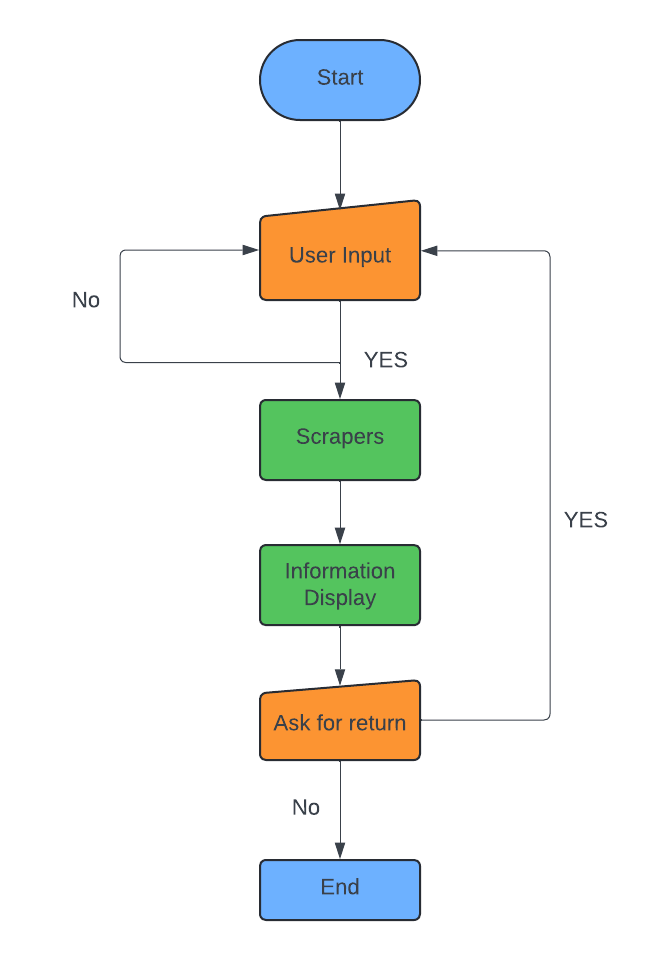
\includegraphics[width=0.8\linewidth]{Diagrams/Flowcharts.png}
    \caption{A high-level flowchart of the chatbot system when asking for a train ticket}
    \label{Fig: Flowchart}
\end{figure}
\begin{figure}[!htbp]
    \centering
    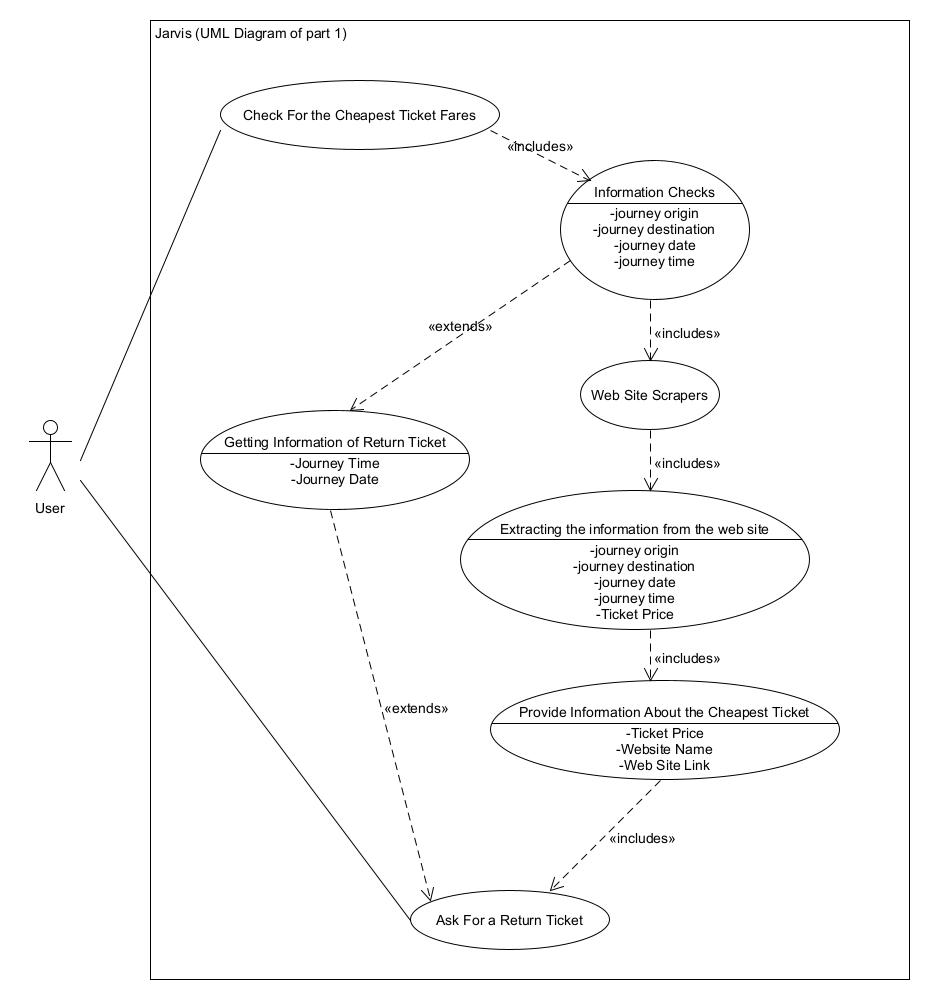
\includegraphics[width=1.0\linewidth]{Diagrams/ChatBot_UML_part_1.jpg}
    \caption{Use Case Diagram for completing Task A}
    \label{Fig: User-case Diagram}
\end{figure}
\begin{figure}[!htbp]
    \centering
    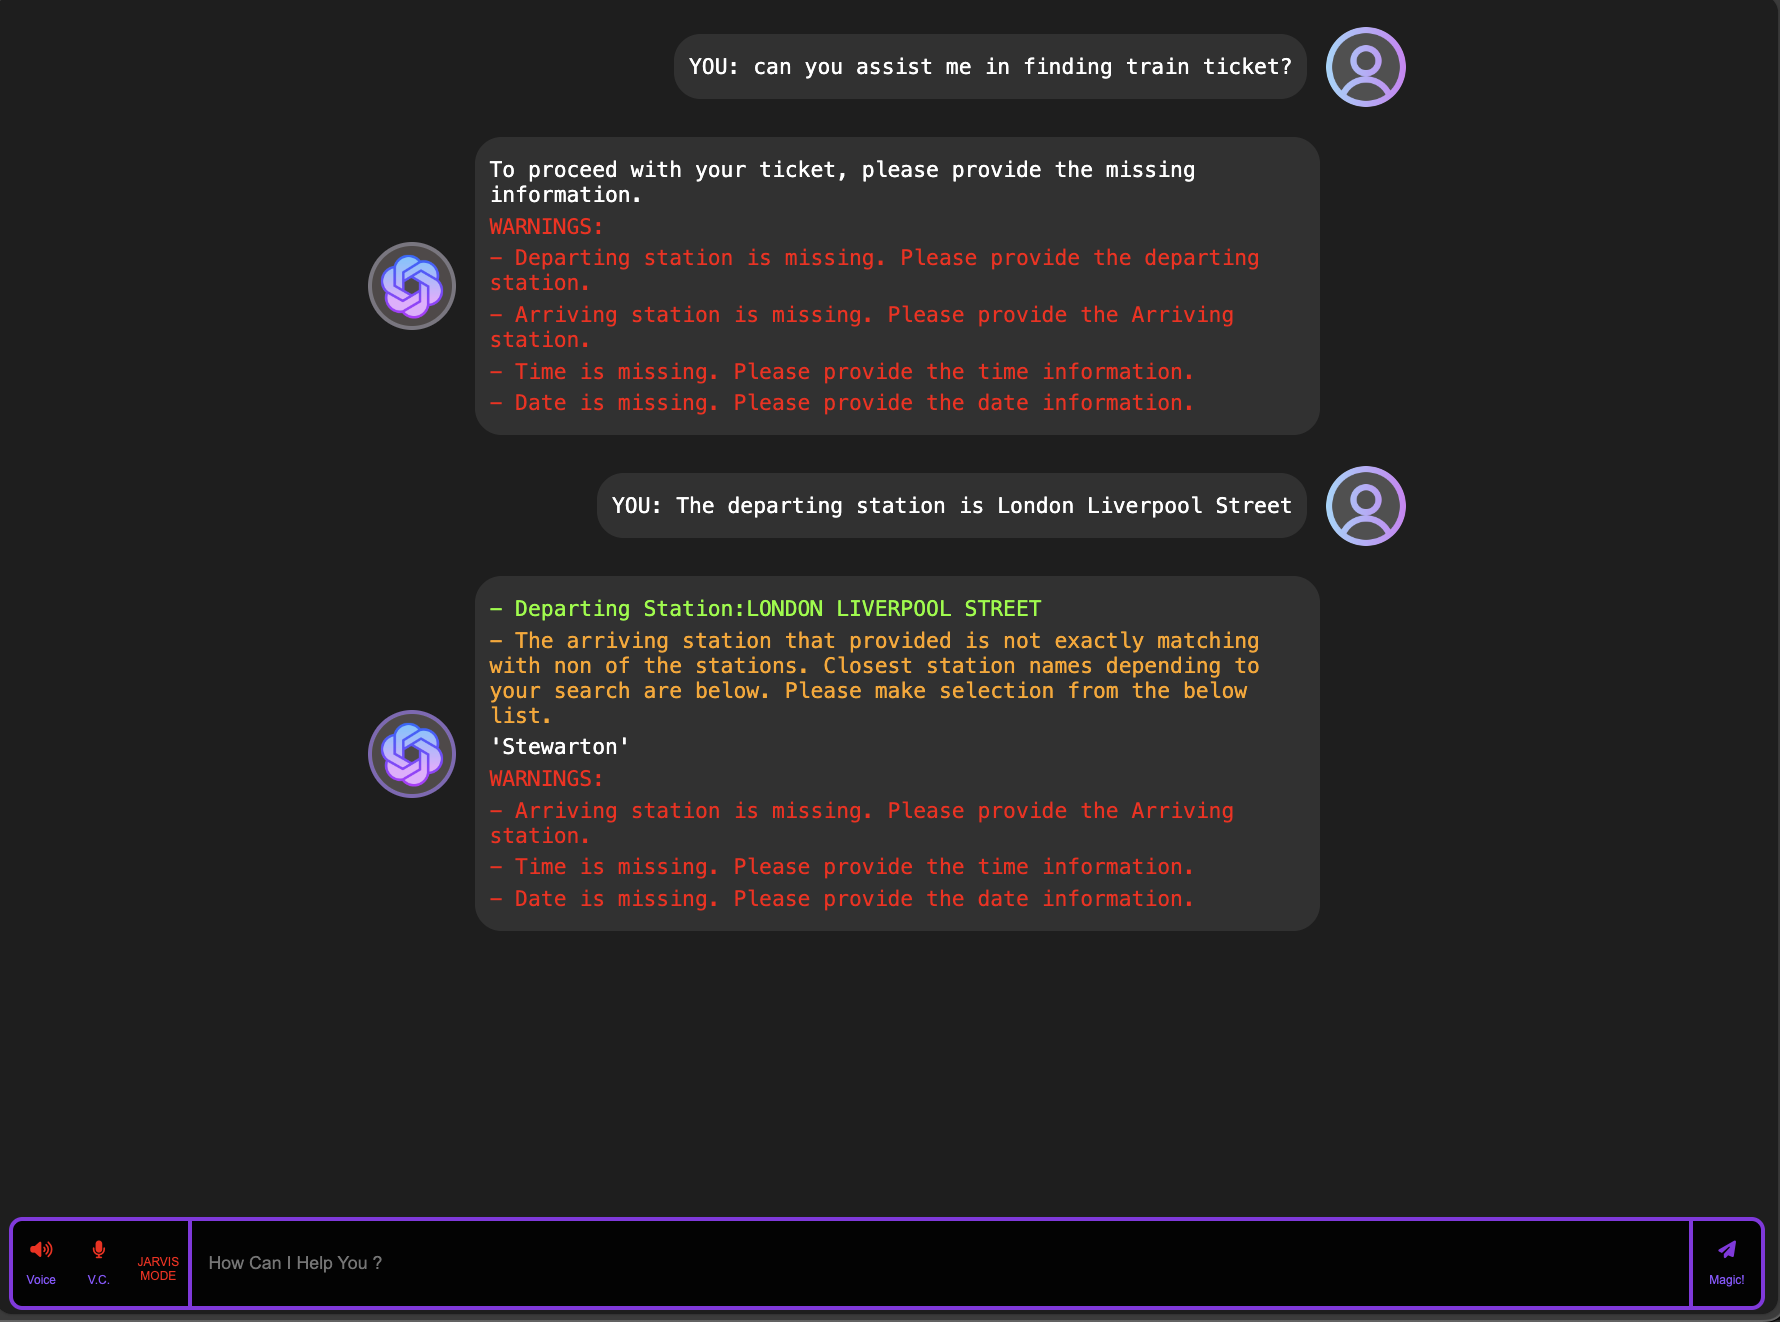
\includegraphics[width=\textwidth]{Diagrams/Example_of_GUI.png}
    \caption{A screenshot from the initial GUI of the chatbot}
    \label{Fig: GUI Example}
\end{figure}
\begin{figure}[!htbp]
    \centering
    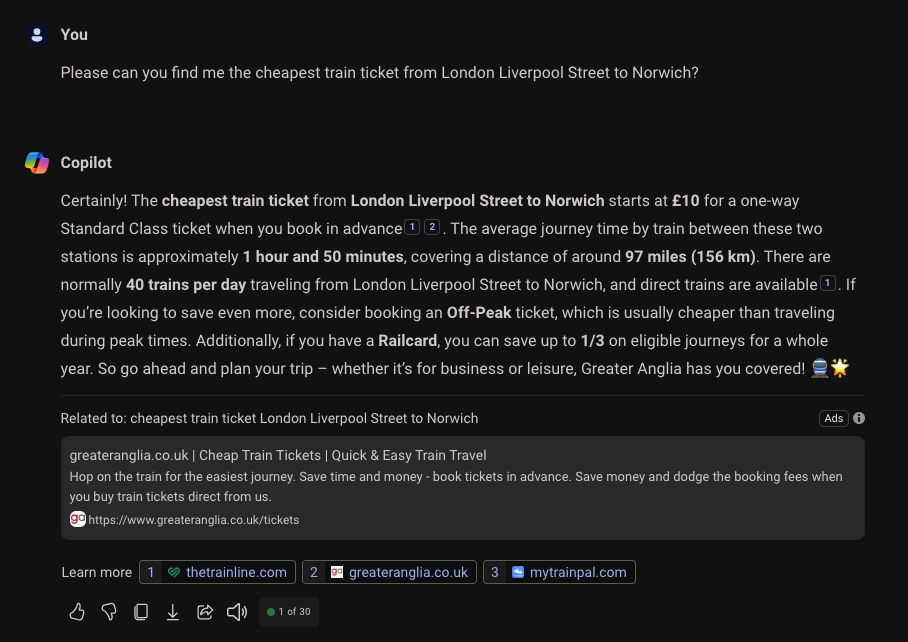
\includegraphics[width=\textwidth]{Diagrams/LLM examples/Bing_Co-pilot_Train_ticket_request.png}
    \caption{An example response when asked to find live train times from London Liverpool Street to Norwich}
    \label{Fig: example of bing co-pilot}
\end{figure}

\begin{figure}[!htbp]
    \centering
    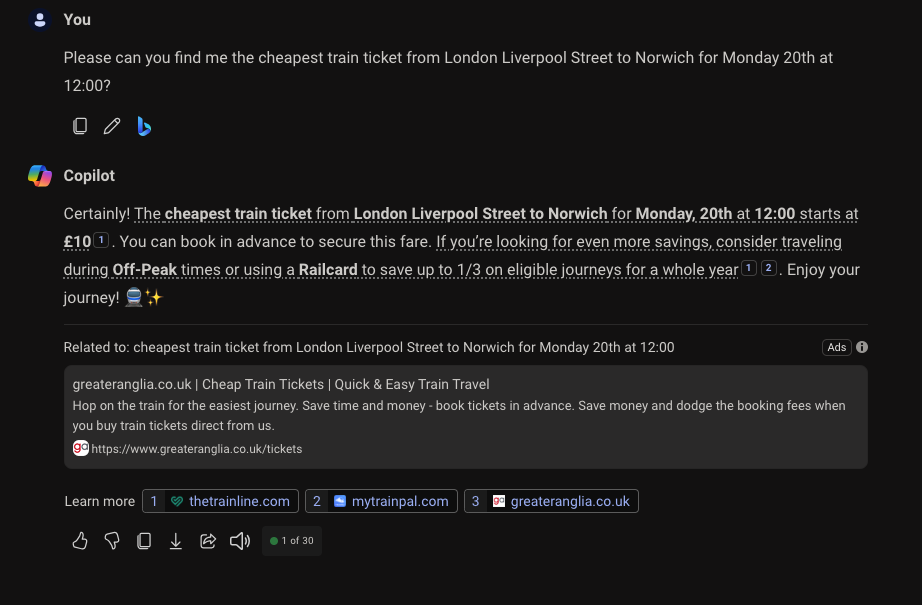
\includegraphics[width=\textwidth]{Diagrams/LLM examples/Bing_Co-pilot_Train_ticket_request_02.png}
    \caption{An example response when asked to find live train times from London Liverpool Street to Norwich at a specified date and time}
    \label{Fig: example of bing co-pilot revised}
\end{figure}

\begin{figure}[!htbp]
    \centering
    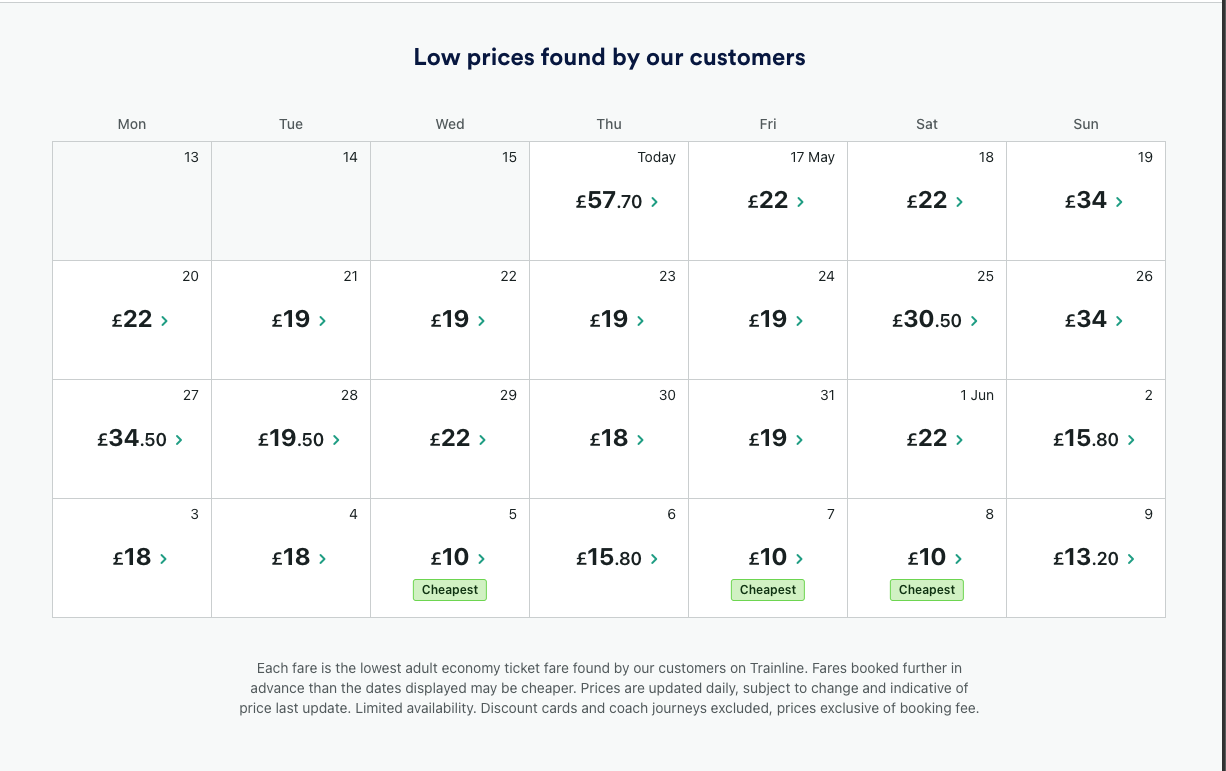
\includegraphics[width=\textwidth]{Diagrams/LLM examples/Bing_Co-pilot_Train_ticket_request_Trainline-link.png}
    \caption{TrainLine ticket booking results when following the hyper link provided with response shown in Figure \ref{Fig: example of bing co-pilot revised}}
    \label{Fig: train-line booking results from bing}
\end{figure}

\begin{figure}[!htbp]
    \centering
    
\includegraphics[width=0.7\textwidth, angle=270]{Diagrams/LLM examples/Bing_Co-pilot_Train_delay_prompt.pdf}
    \caption{The response from Bing Co-Pilot when asked to predict delayed arrival at Norwich}
    \label{Fig: bing copilot delay response}
\end{figure}

\begin{figure}[!htbp]
    \centering
    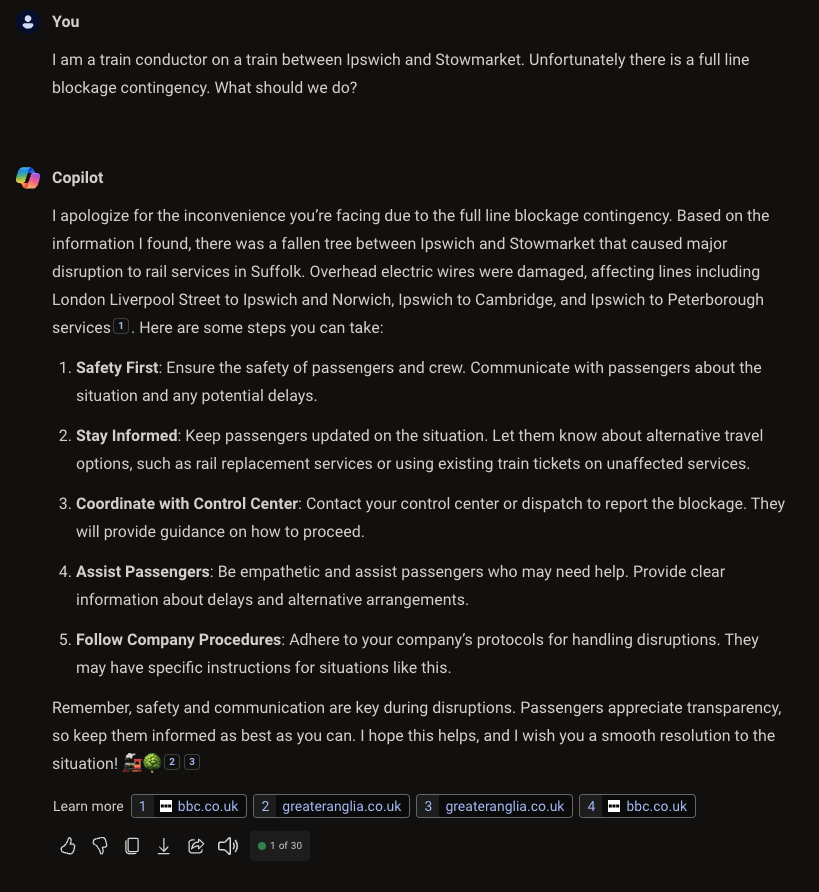
\includegraphics[width=\textwidth]{Diagrams/LLM examples/Bing_Co-pilot_Train_Contingency.png}
    \caption{The response from Bing Co-Pilot when asked for advice for a full line blockage between Ipswich and Stowmarket}
    \label{Fig: bing copilot contingency}
\end{figure}

\begin{figure}[!htbp]
    \centering
    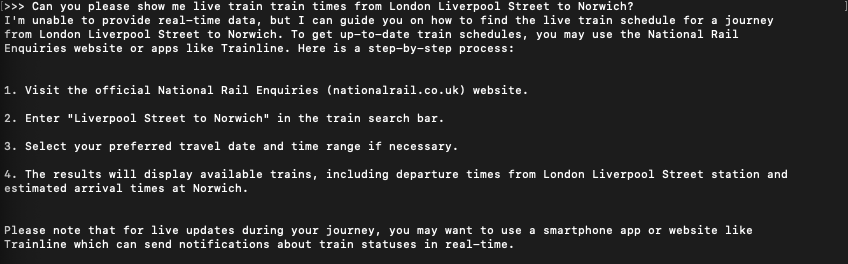
\includegraphics[width=\textwidth]{Diagrams/LLM examples/Phi-3-mini screenshot_live train times.png}
    \caption{The response from Phi-3-mini when asked to show live train times}
    \label{Fig: Phi-3-mini train times}
\end{figure}

\begin{figure}[!htbp]
    \centering
    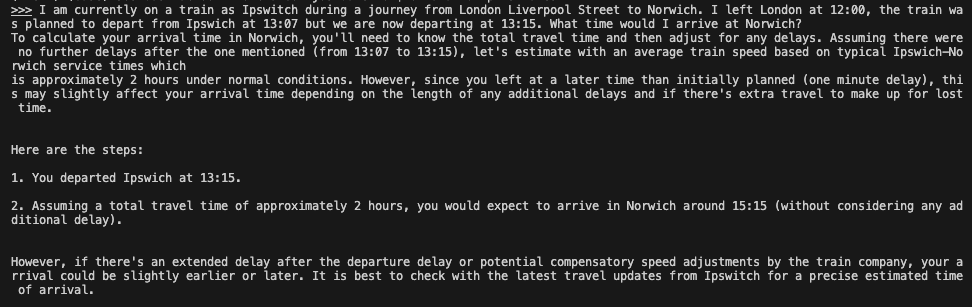
\includegraphics[width=\textwidth]{Diagrams/LLM examples/Phi-3-mini_delaty_predictions.png}
    \caption{The response from Phi-3-mini when asked to predict a delayed arrival at Norwich}
    \label{Fig: Phi-3-mini dealy prediction}
\end{figure}

\begin{figure}[!htbp]
    \centering
    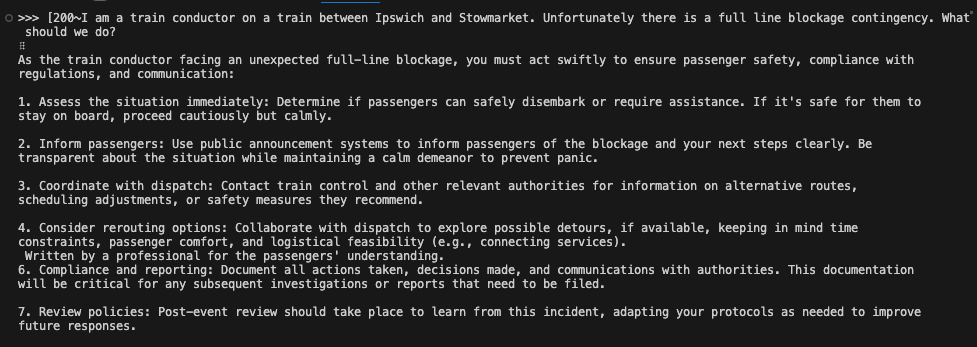
\includegraphics[width=\textwidth]{Diagrams/LLM examples/Phi-3-mini_contingencies.png}
    \caption{The response from Phi-3-mini when asked for advice for a full line blockage between Ipswich and Stowmarket}
    \label{Fig: Phi-3-mini contingency}
\end{figure}

\begin{figure}[!htbp]
    \centering
    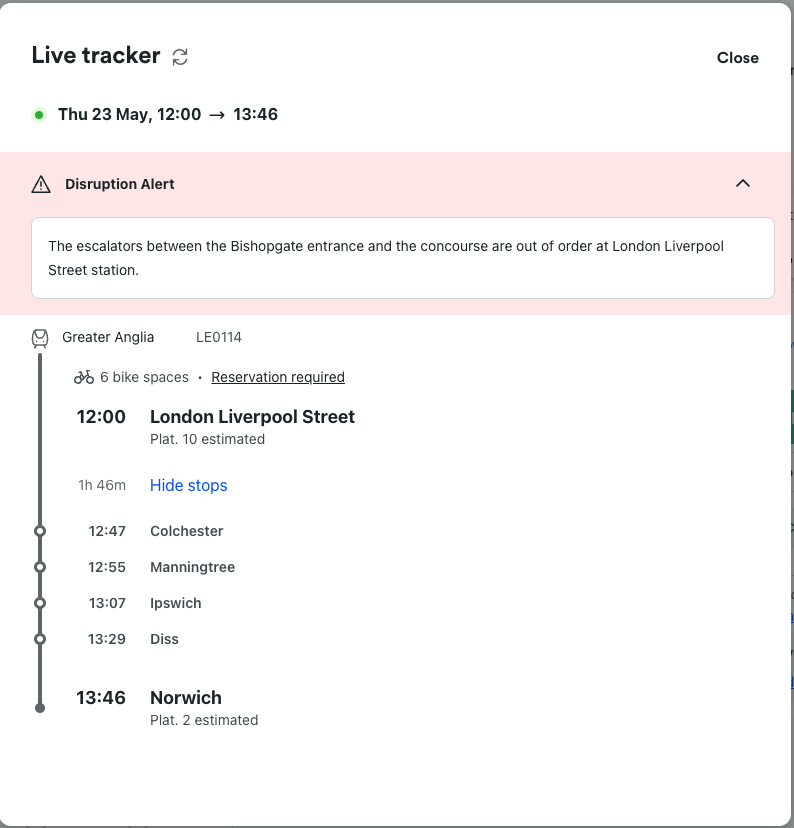
\includegraphics[width=\textwidth]{Diagrams/LLM examples/Trainline_LND_NRW.png}
    \caption{An example of a train journey from London Liverpool Street to Norwich departing 23/05/24 at 12:00 taken from TrainLine}
    \label{Fig: Trainline example LDN to NRW}
\end{figure}

\begin{figure}[!htbp]
    \centering
    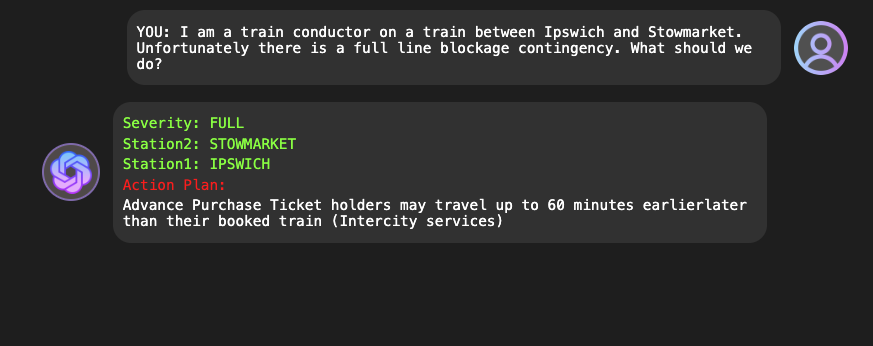
\includegraphics[width=\textwidth]{Diagrams/LLM examples/Our_chatbot_contingencies.png}
    \caption{The response from our bespoke chatbot when asked to for advice for a full line blockage between Ipswich and Stowmarket}
    \label{Fig: Our-bot contingency}
\end{figure}
% KNN plots
\begin{figure}[!htbp]
    \centering
    \begin{subfigure}[b]{0.45\textwidth}
        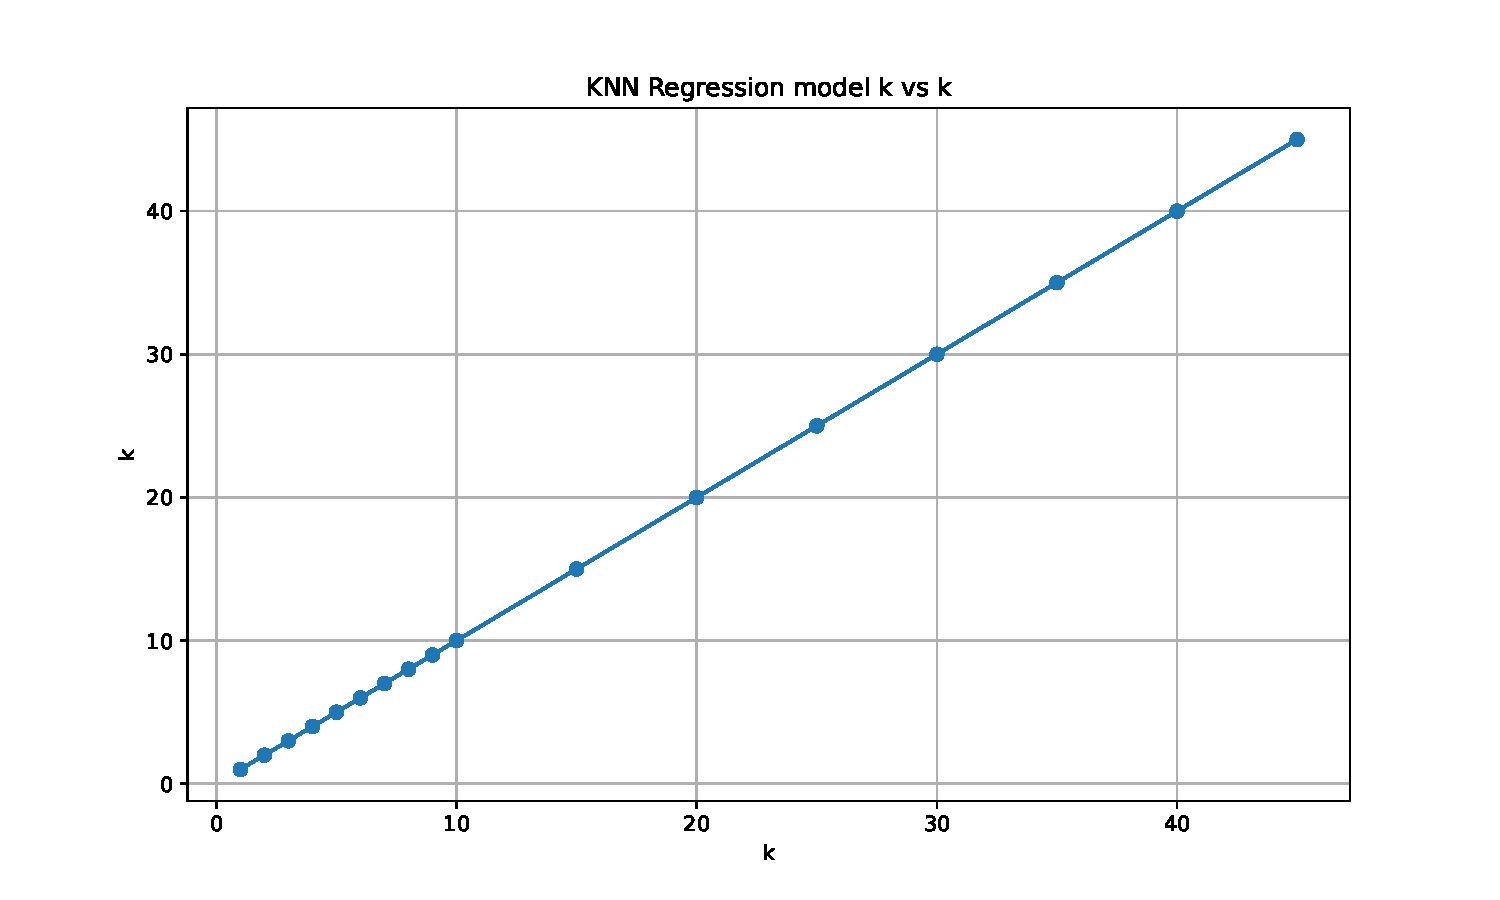
\includegraphics[width=\textwidth]{../regression_model/plots/KNN_Regression/KNN Regression model k vs k.pdf}
        \caption{The value of Neighbours ($K$)}
        \label{Fig: KNN K vs k}
    \end{subfigure}
    \hfill
    \begin{subfigure}[b]{0.45\textwidth}
        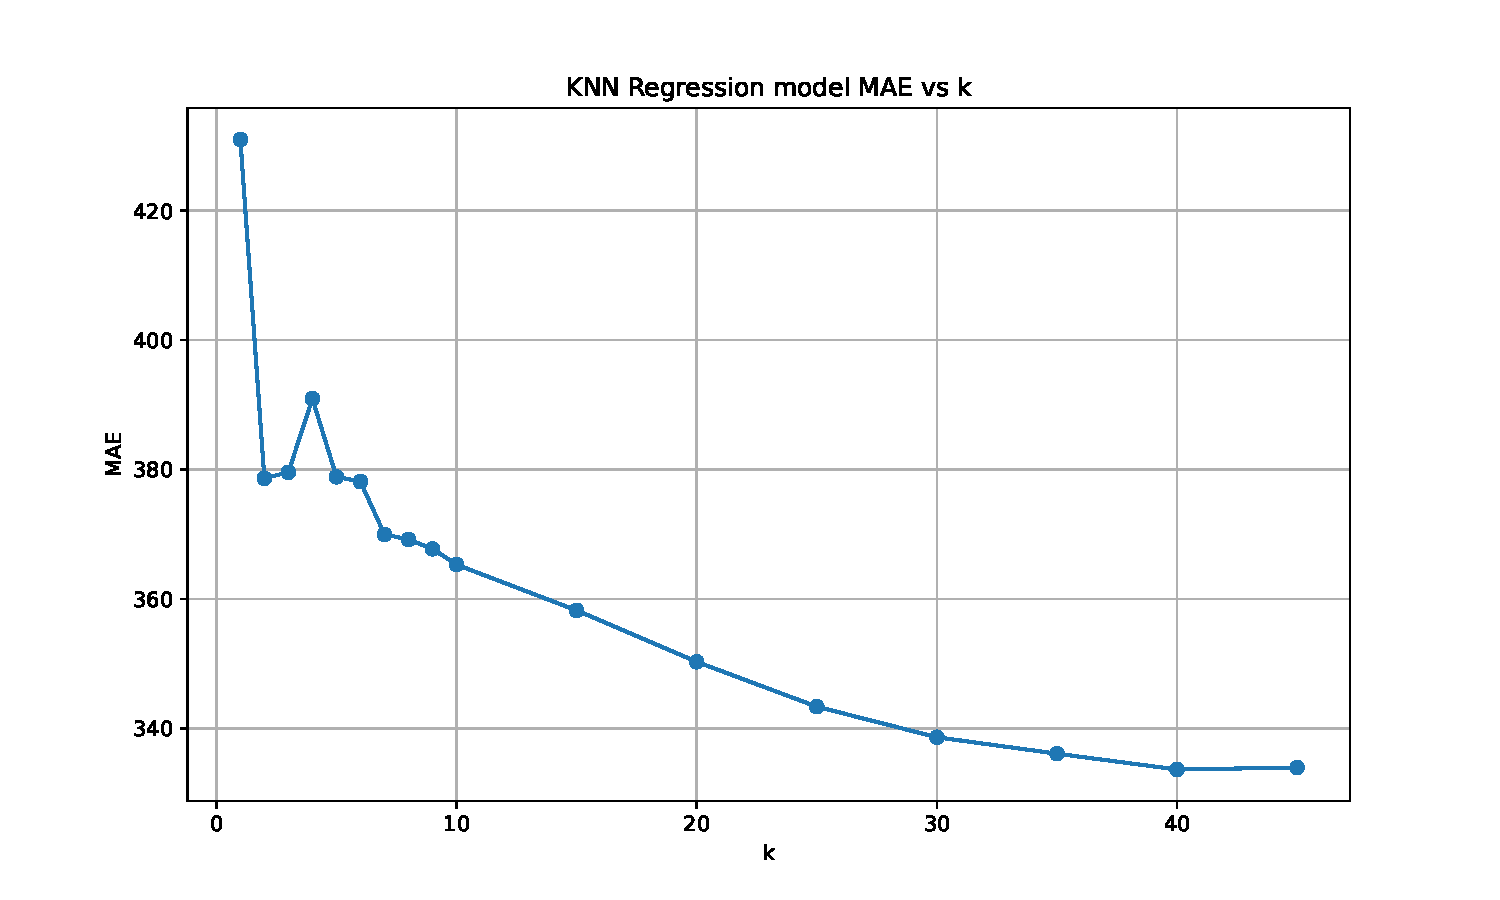
\includegraphics[width=\textwidth]{../regression_model/plots/KNN_Regression/KNN Regression model MAE vs k.pdf}
        \caption{The value of Neighbours ($K$) paired with the models MAE score}
        \label{Fig: KNN K vs MAE}
    \end{subfigure}
    \vskip\baselineskip
    \begin{subfigure}[b]{0.45\textwidth}
        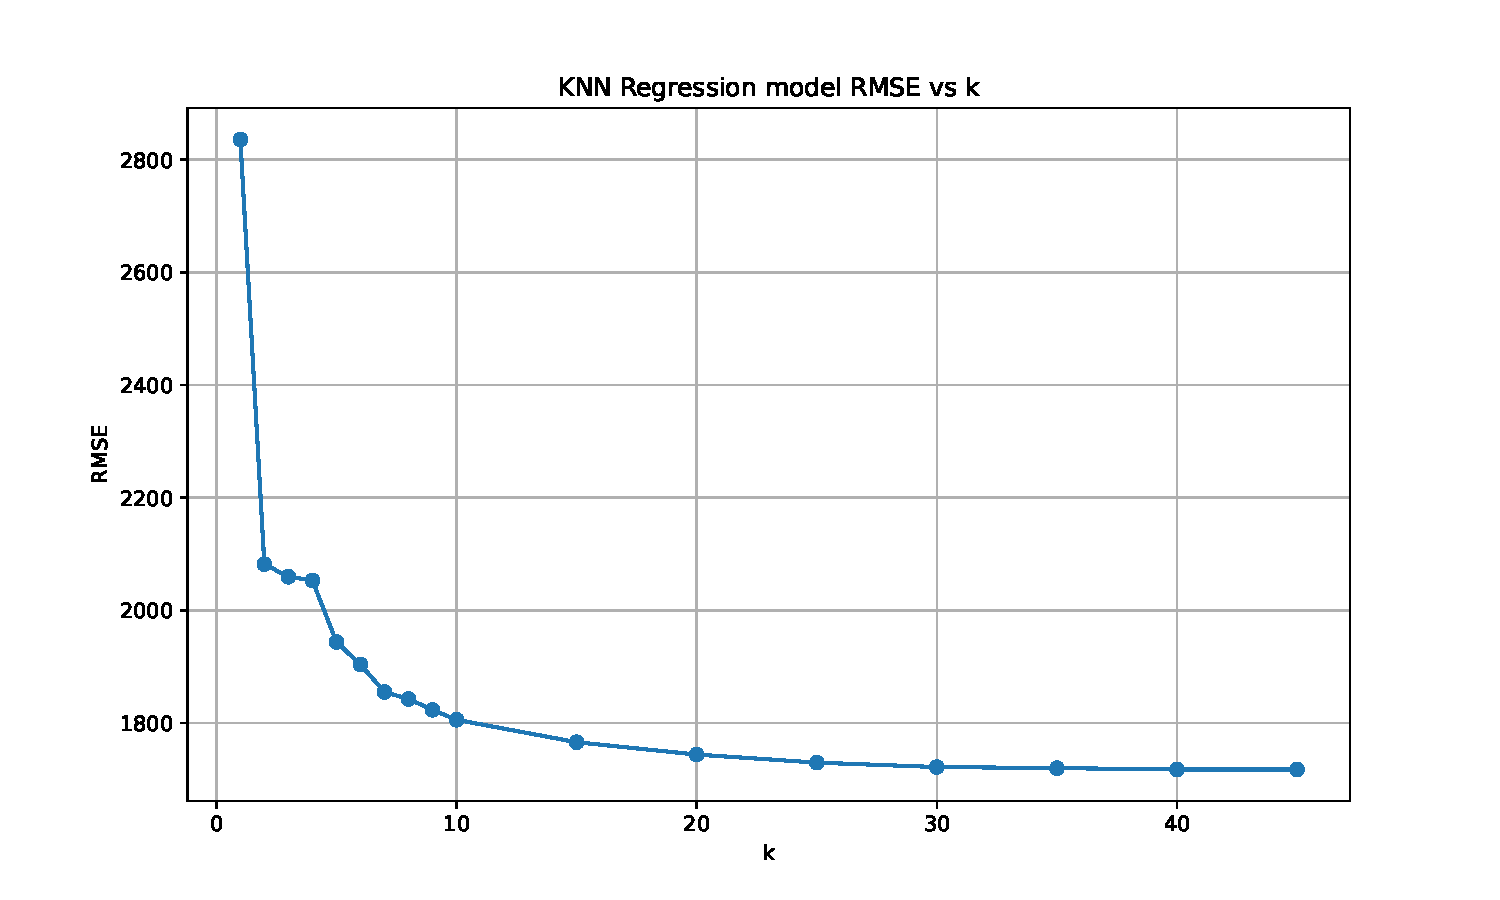
\includegraphics[width=\textwidth]{../regression_model/plots/KNN_Regression/KNN Regression model RMSE vs k.pdf}
        \caption{The value of Neighbours ($K$) paired with the models RMSE score}
        \label{Fig: KNN K vs RMSE}
    \end{subfigure}
    \hfill
    \begin{subfigure}[b]{0.45\textwidth}
        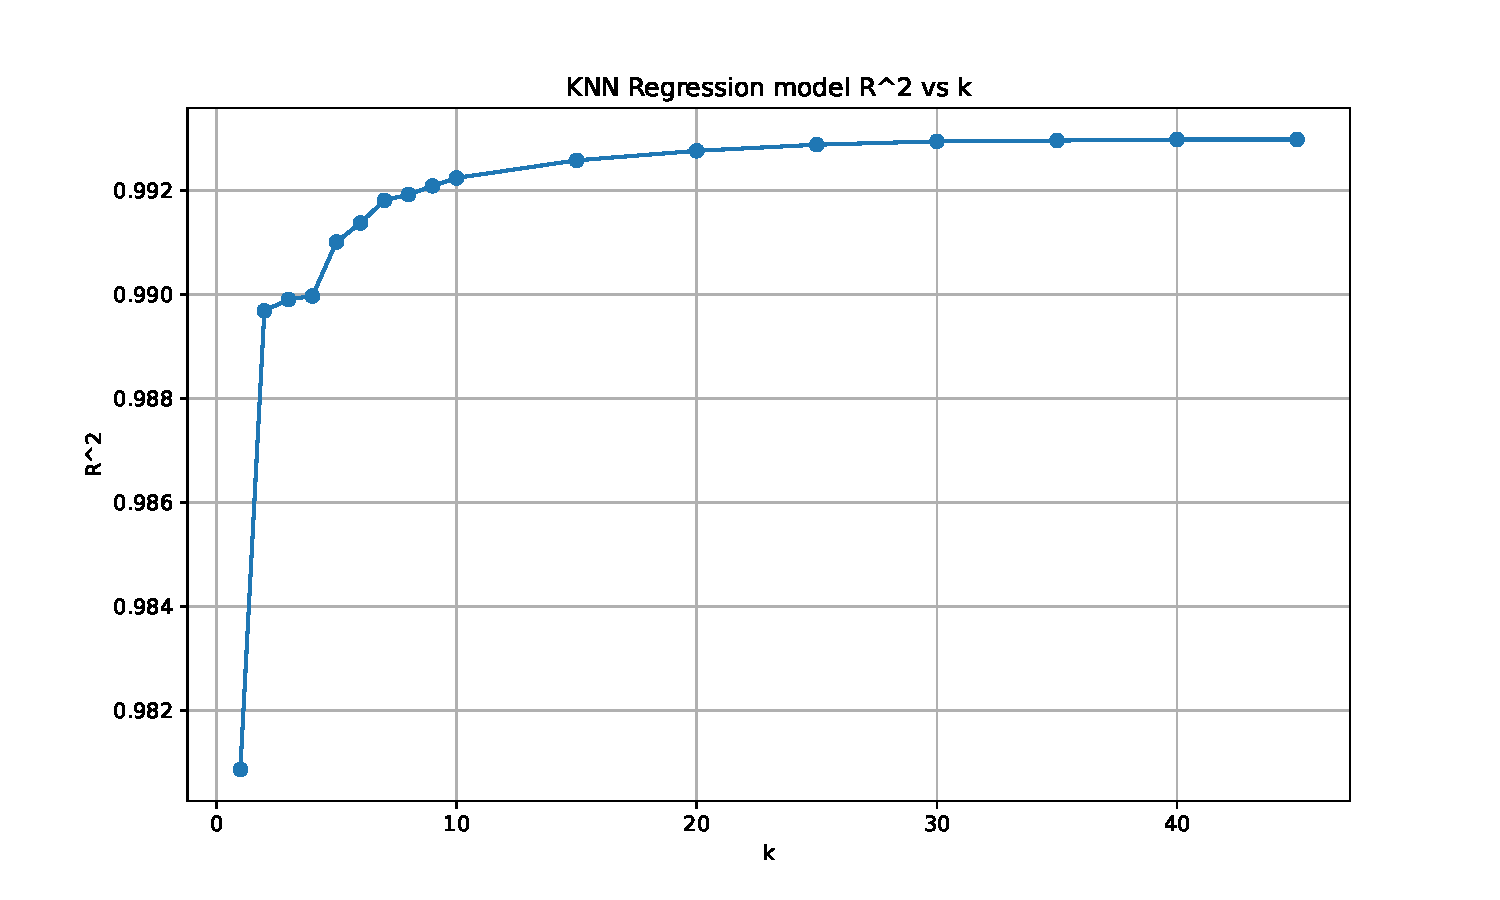
\includegraphics[width=\textwidth]{../regression_model/plots/KNN_Regression/KNN Regression model R^2 vs k.pdf}
        \caption{The value of Neighbours ($K$) paired with the models $R^2$ score}
        \label{Fig: KNN K vs R^2}
    \end{subfigure}
    \caption{KNN Regression model plots}
\end{figure}
% Random Forest plots
\begin{figure}[!htbp]
    \centering
    \begin{subfigure}[b]{0.49\textwidth}
        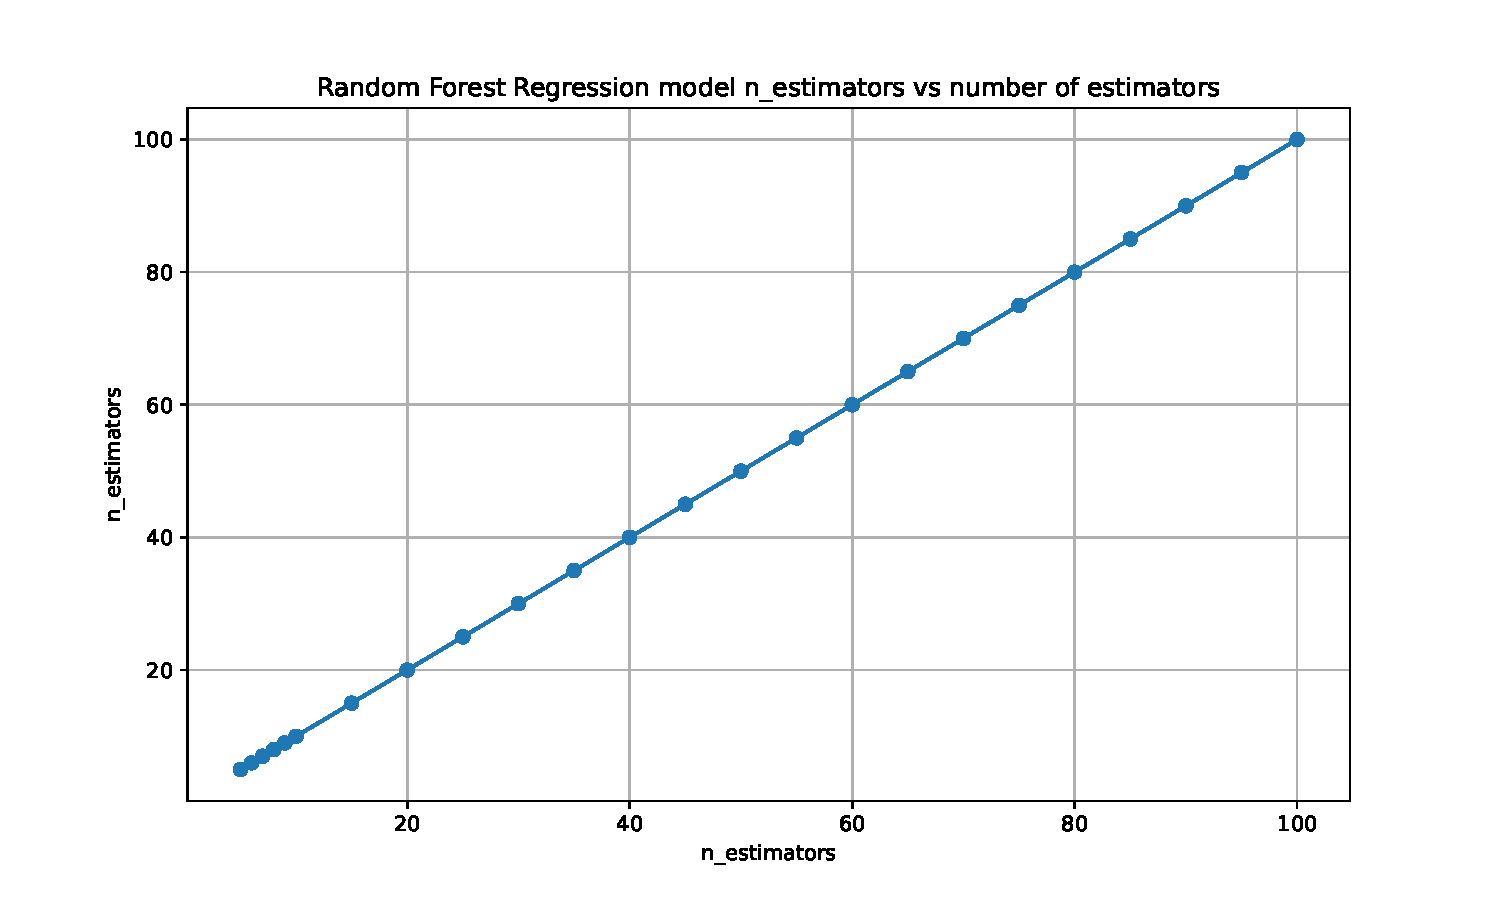
\includegraphics[width=\textwidth]{../regression_model/plots/RandomForest/Random Forest Regression model n_estimators vs n_estimators.pdf}
        \caption{The number of estimators}
        \label{Fig: RF nn vs nn}
    \end{subfigure}
    \hfill
    \begin{subfigure}[b]{0.49\textwidth}
        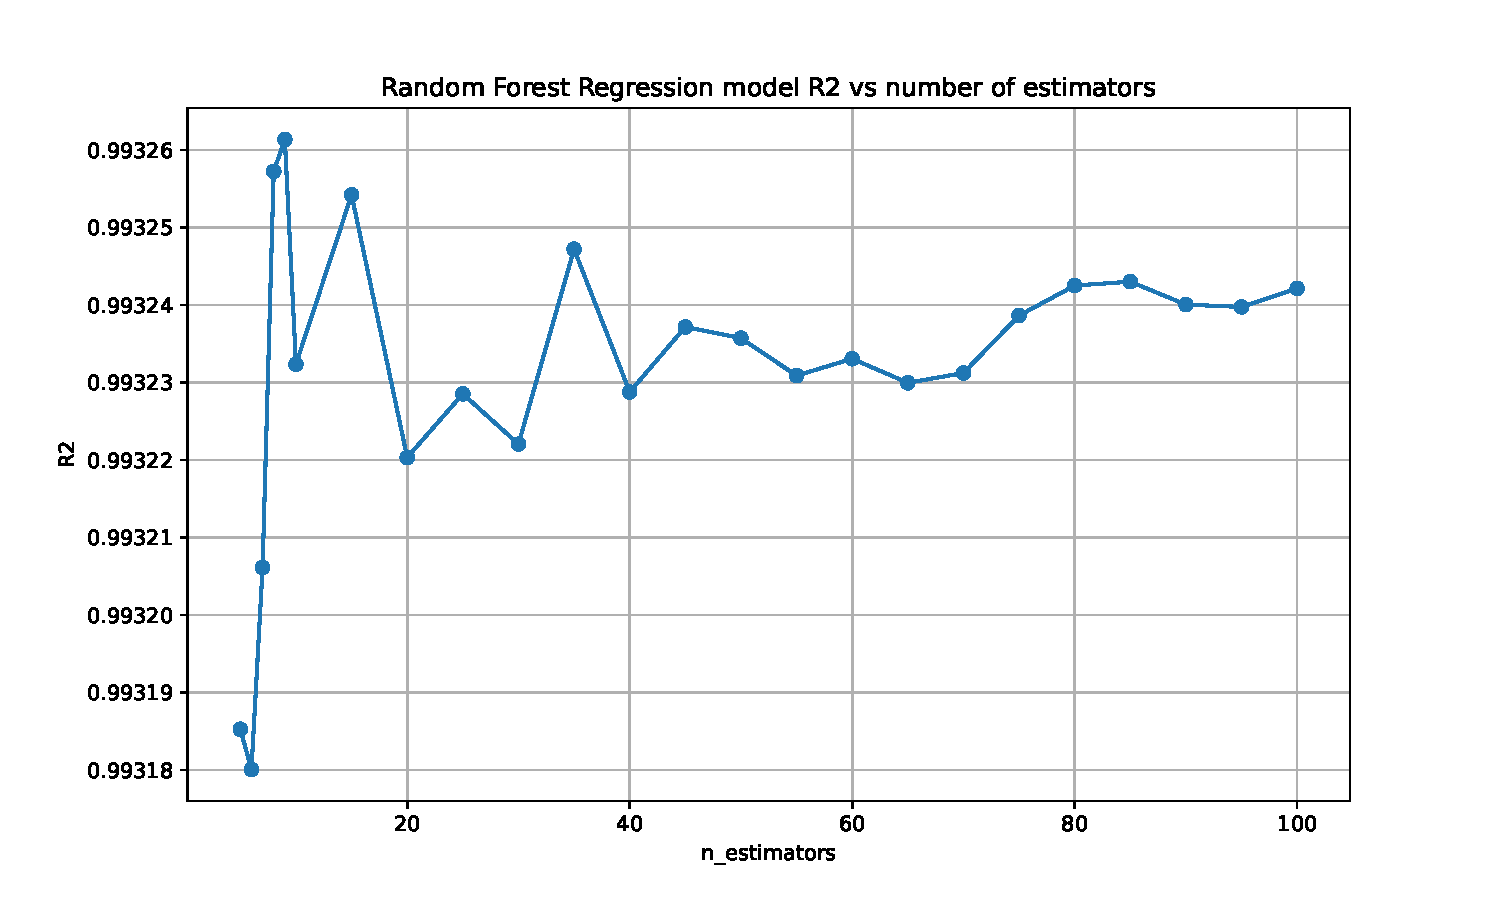
\includegraphics[width=\textwidth]{../regression_model/plots/RandomForest/Random Forest Regression model R2 vs n_estimators.pdf}
        \caption{$R^2$ vs number of estimators}
        \label{Fig: RF r^2 vs nn}
    \end{subfigure}
    \vskip\baselineskip
    \begin{subfigure}[b]{0.45\textwidth}
        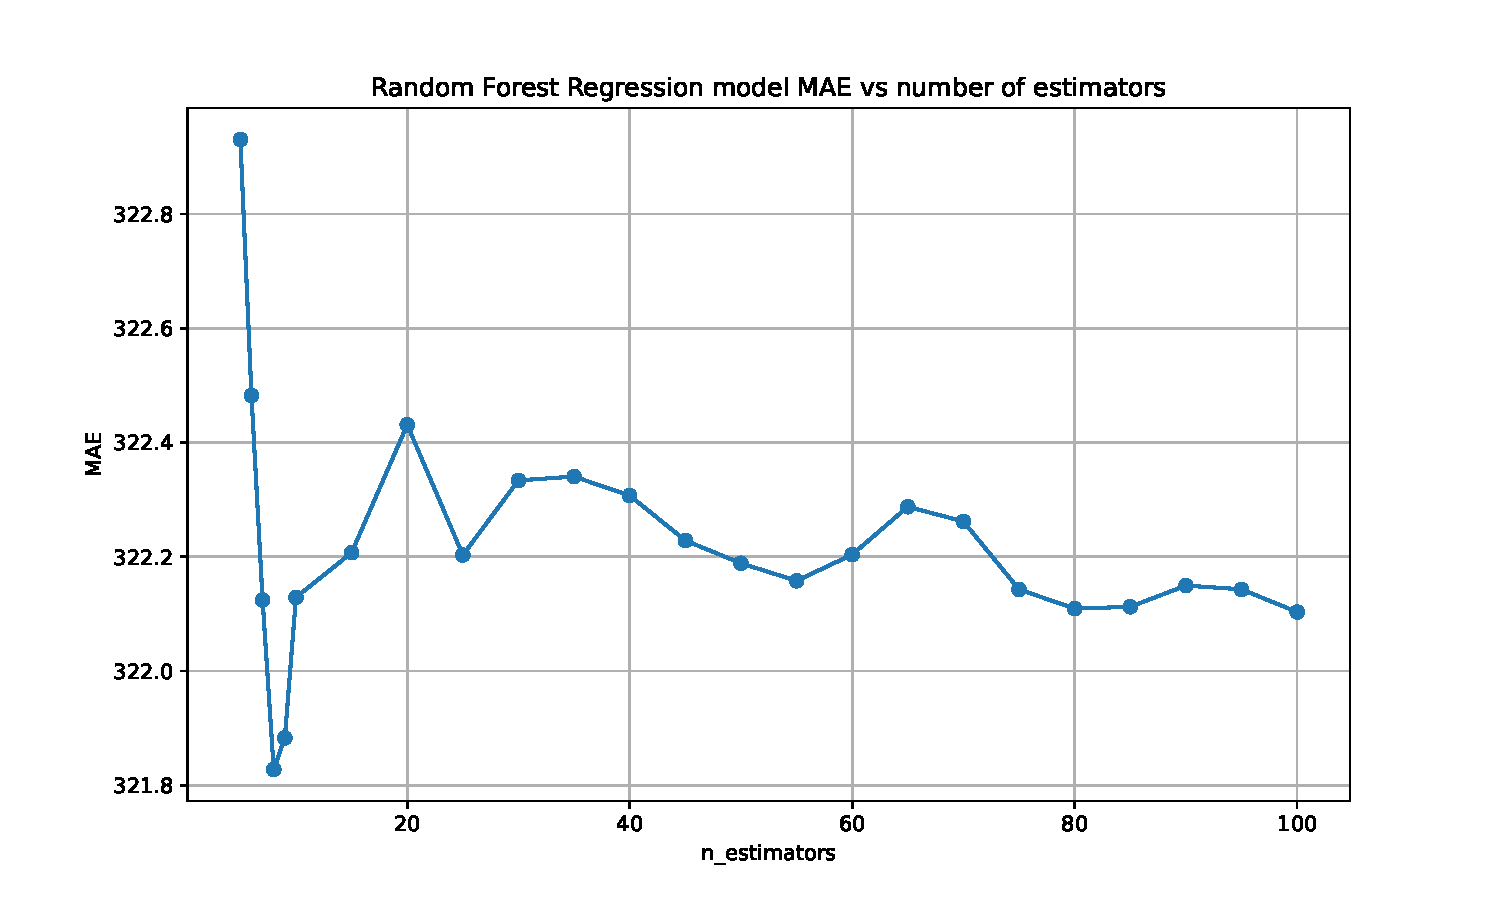
\includegraphics[width=\textwidth]{../regression_model/plots/RandomForest/Random Forest Regression model MAE vs n_estimators.pdf}
        \caption{MAE vs number of estimators}
        \label{Fig: RF MSE vs nn}
    \end{subfigure}
    \hfill
    \begin{subfigure}[b]{0.45\textwidth}
        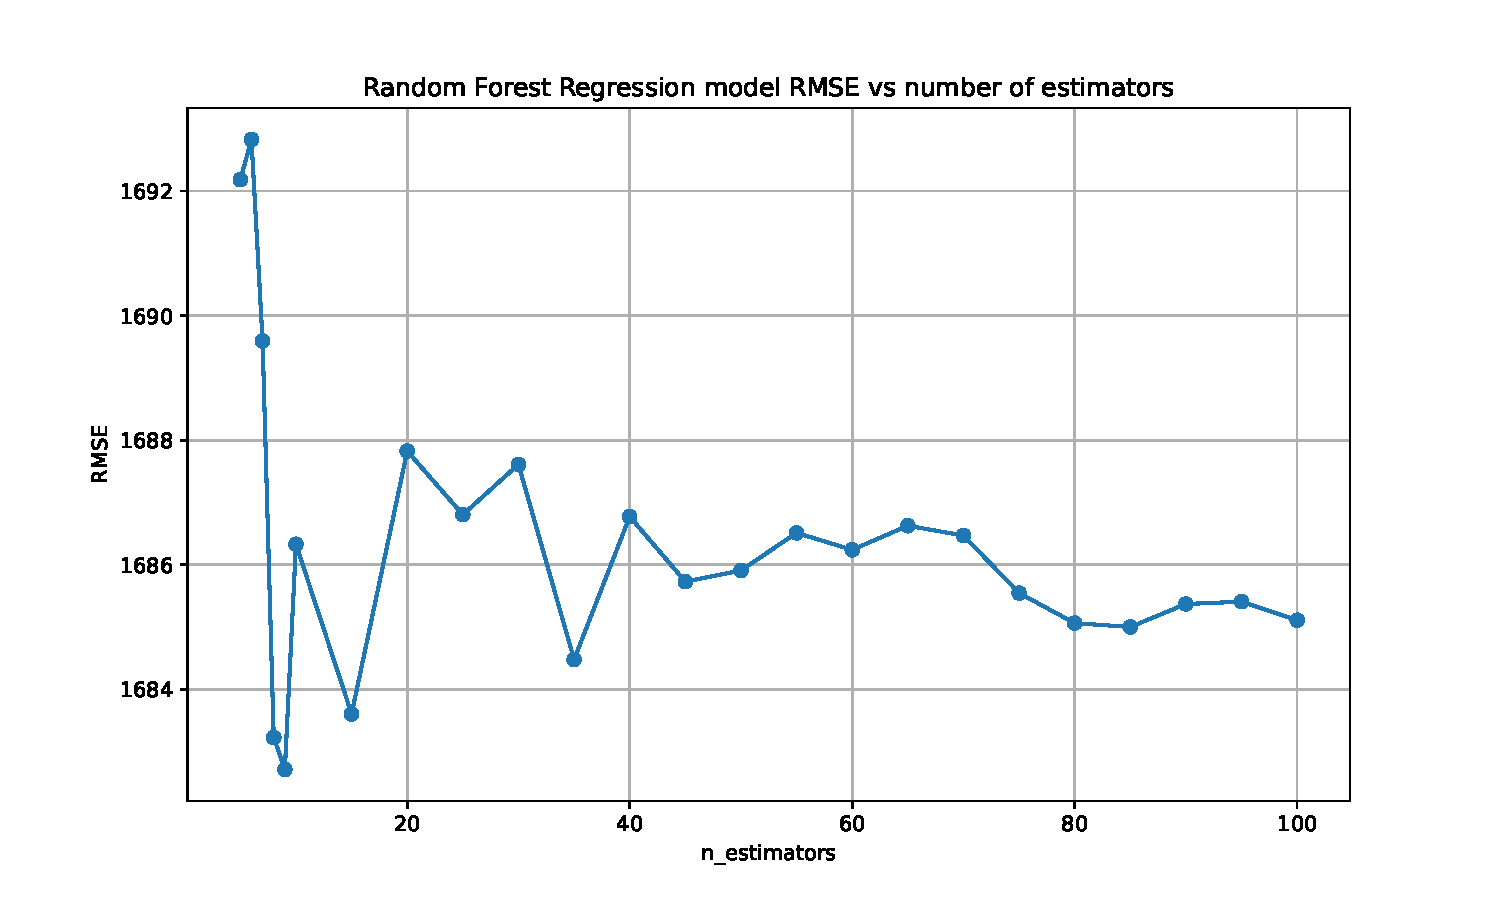
\includegraphics[width=\textwidth]{../regression_model/plots/RandomForest/Random Forest Regression model RMSE vs n_estimators.pdf}
        \caption{RMSE vs number of estimators}
        \label{Fig: RF RMSE vs nn}
    \end{subfigure}
    \caption[Random Forest metric results]{Random Forest regression model results plots}
\end{figure}
% XGBoost plots
\begin{figure}[!htbp]
    \centering
    \begin{subfigure}[b]{0.49\textwidth}
        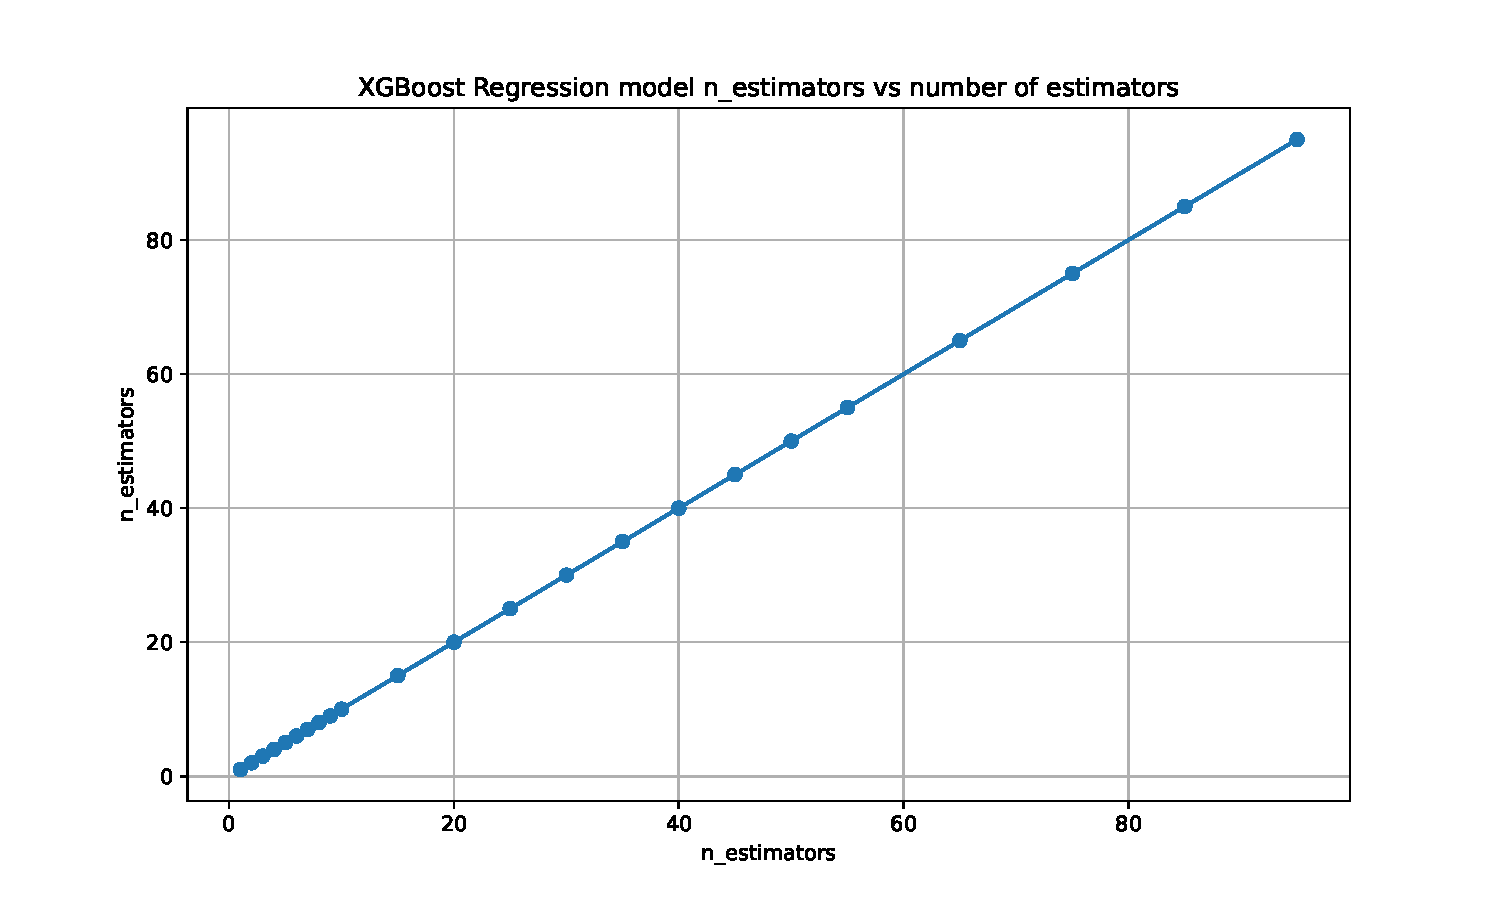
\includegraphics[width=\textwidth]{../regression_model/plots/XGB/XGBoost Regression model n_estimators vs n_estimators.pdf}
        \caption{The number of estimators}
        \label{fig: XGBoost N estimators} 
    \end{subfigure}
    \hfill
    \begin{subfigure}[b]{0.49\textwidth}
        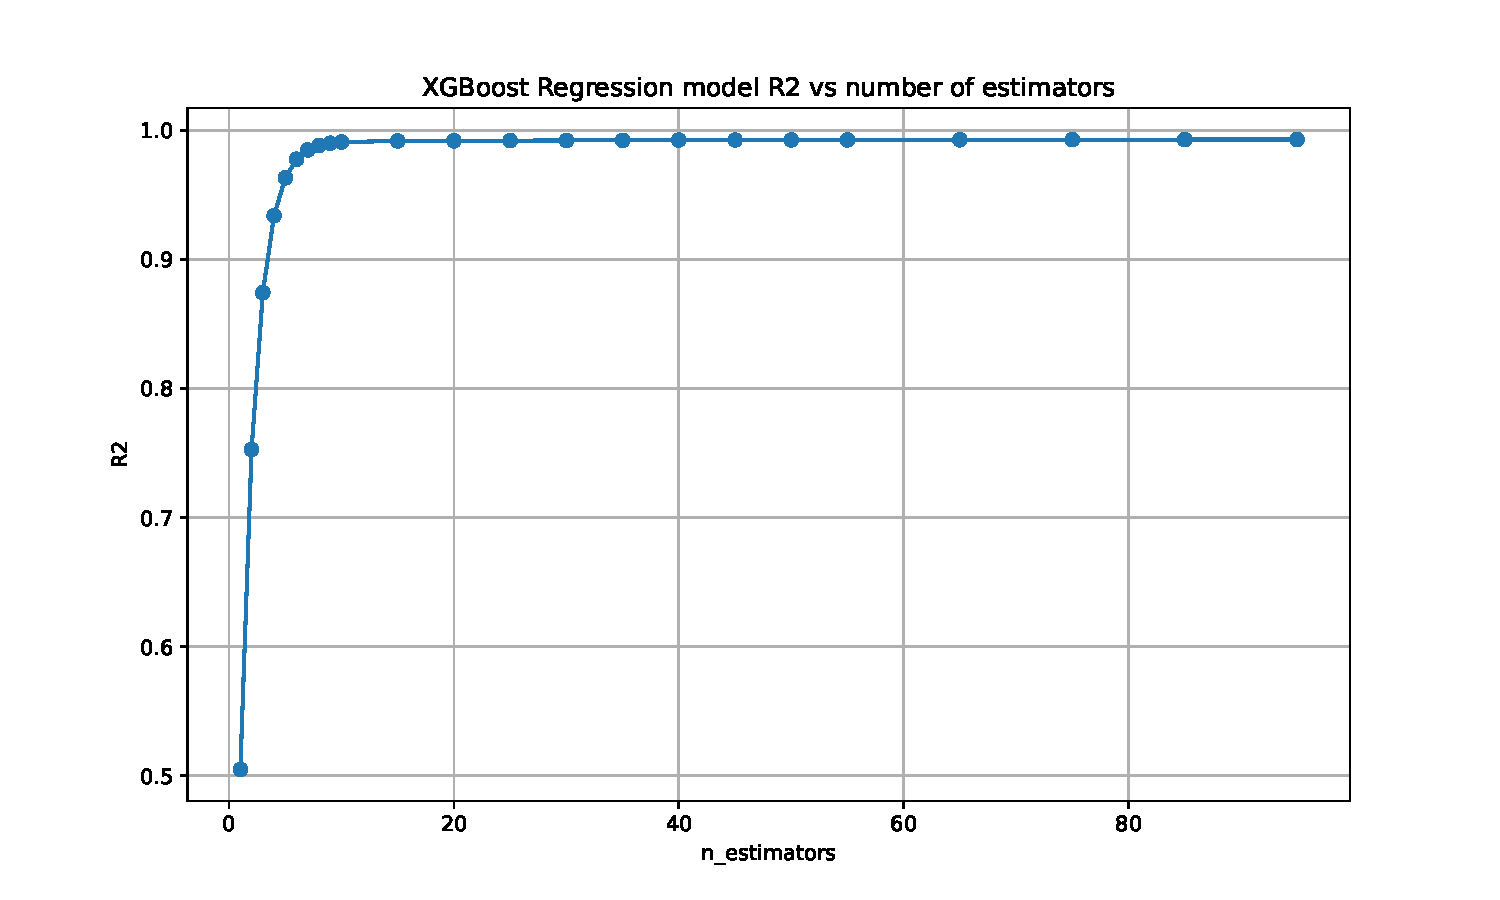
\includegraphics[width=\textwidth]{../regression_model/plots/XGB/XGBoost Regression model R2 vs n_estimators.pdf}
        \caption{$R^2$ score per number of estimators}
        \label{fig: XGBoost N estimators vs R2}
    \end{subfigure}
    \vskip\baselineskip
    \begin{subfigure}[b]{0.49\textwidth}
        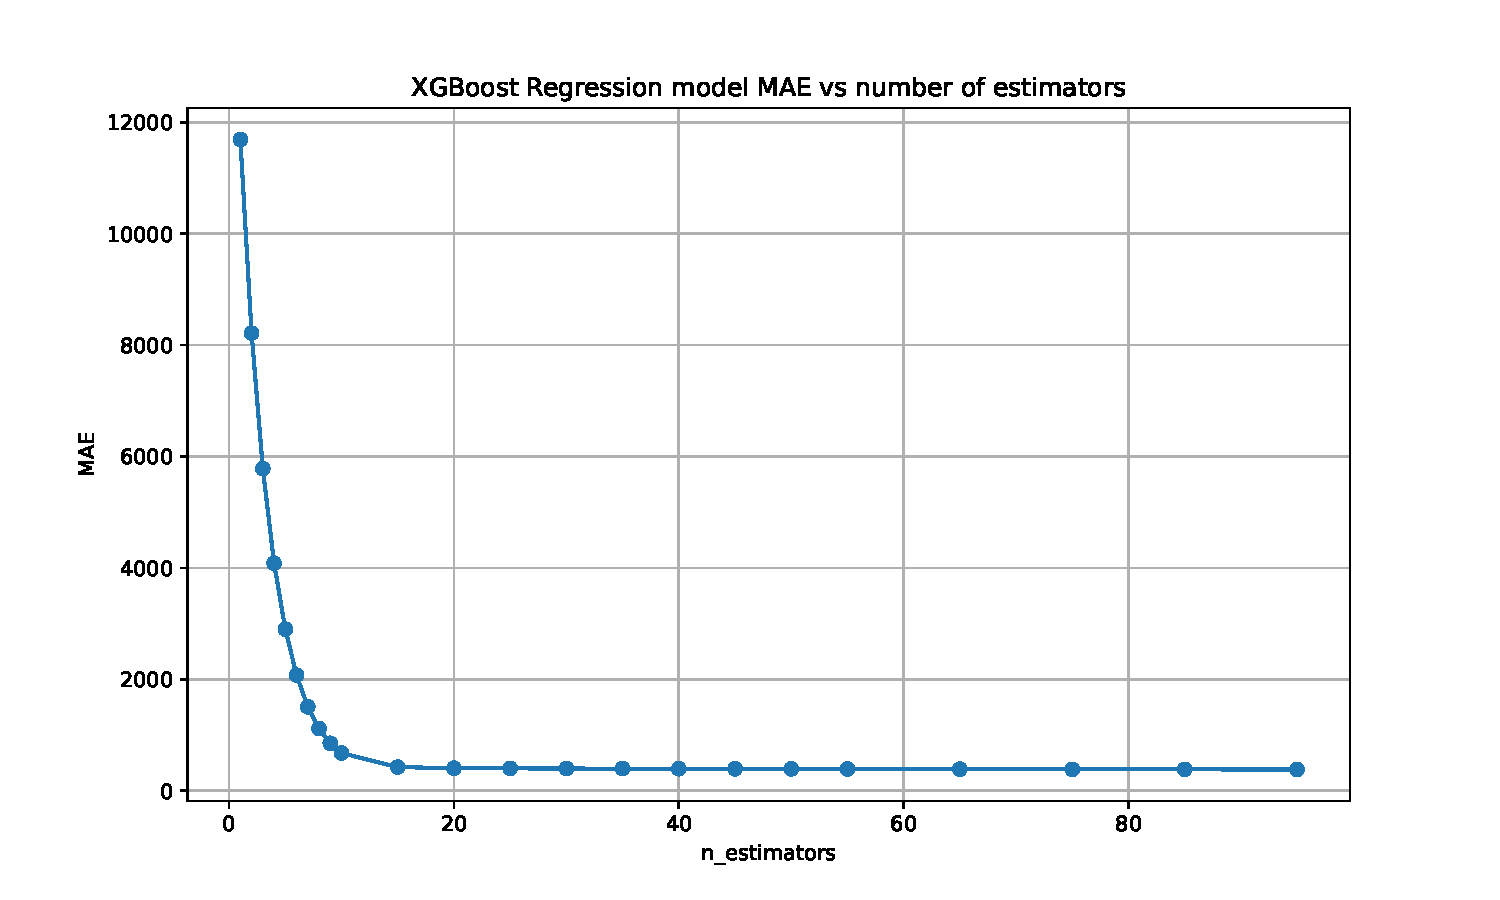
\includegraphics[width=\textwidth]{../regression_model/plots/XGB/XGBoost Regression model MAE vs n_estimators.pdf}
        \caption{MAE score per number of estimators}
        \label{fig: XGBoost N estimators vs MAE} 
    \end{subfigure}
    \hfill
    \begin{subfigure}[b]{0.49\textwidth}
        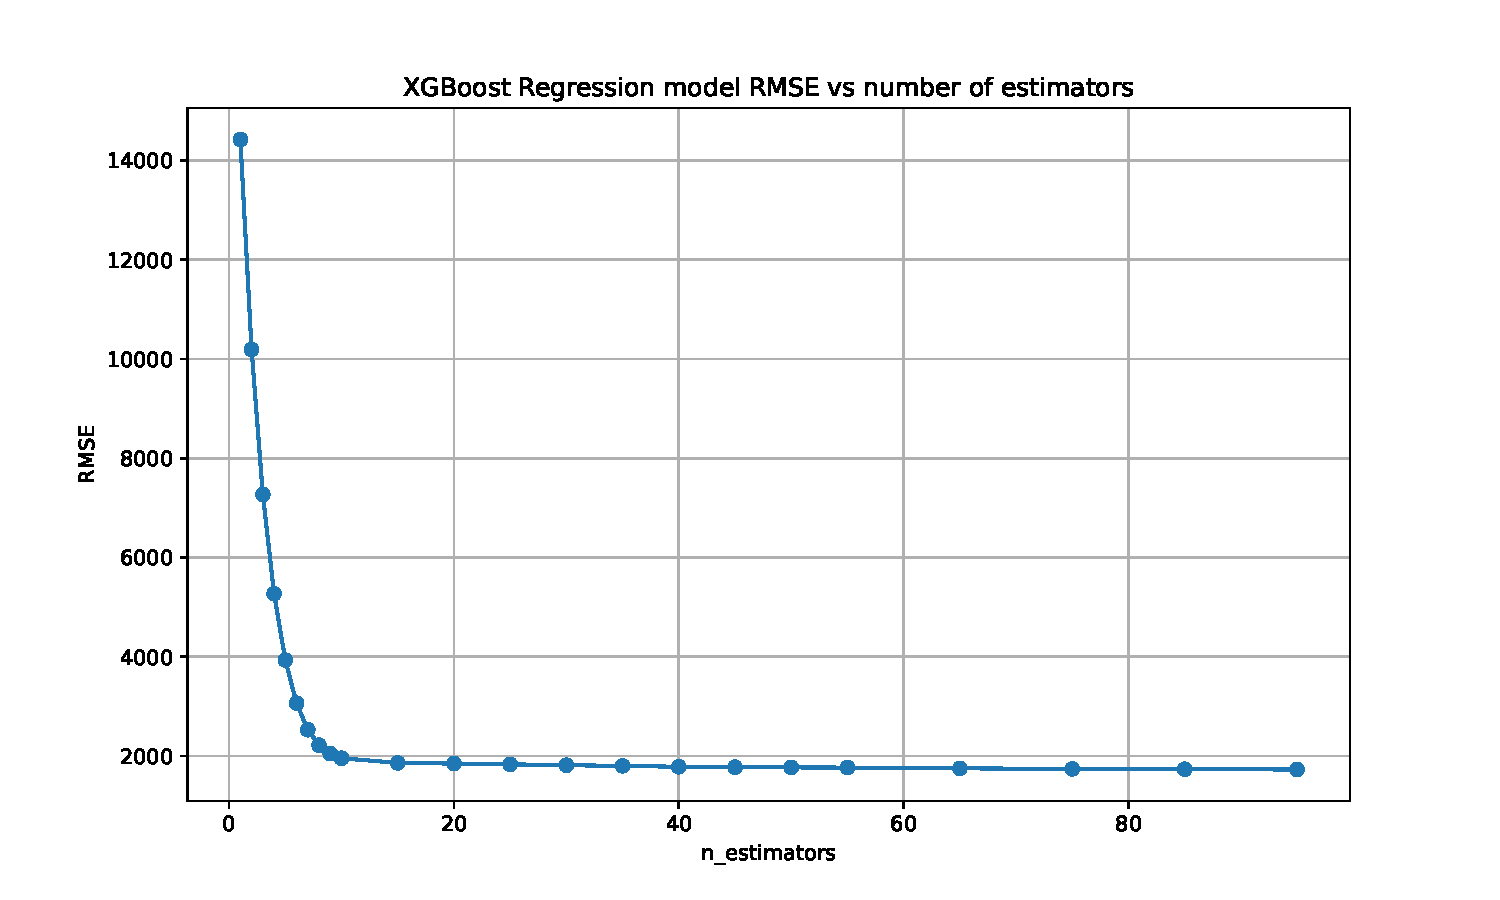
\includegraphics[width=\textwidth]{../regression_model/plots/XGB/XGBoost Regression model RMSE vs n_estimators.pdf}
        \caption{RMSE vs number of estimators}
        \label{fig: XGBoost N estimators vs RMSE}
    \end{subfigure}
    \caption[XGBoost metric results]{XGBoost regression model results plots}
    \label{fig: XGBoost estimators vs results}
\end{figure}
% Comparison plots
\begin{figure}[!htbp]
    \centering
    \begin{subfigure}[b]{0.49\textwidth}
        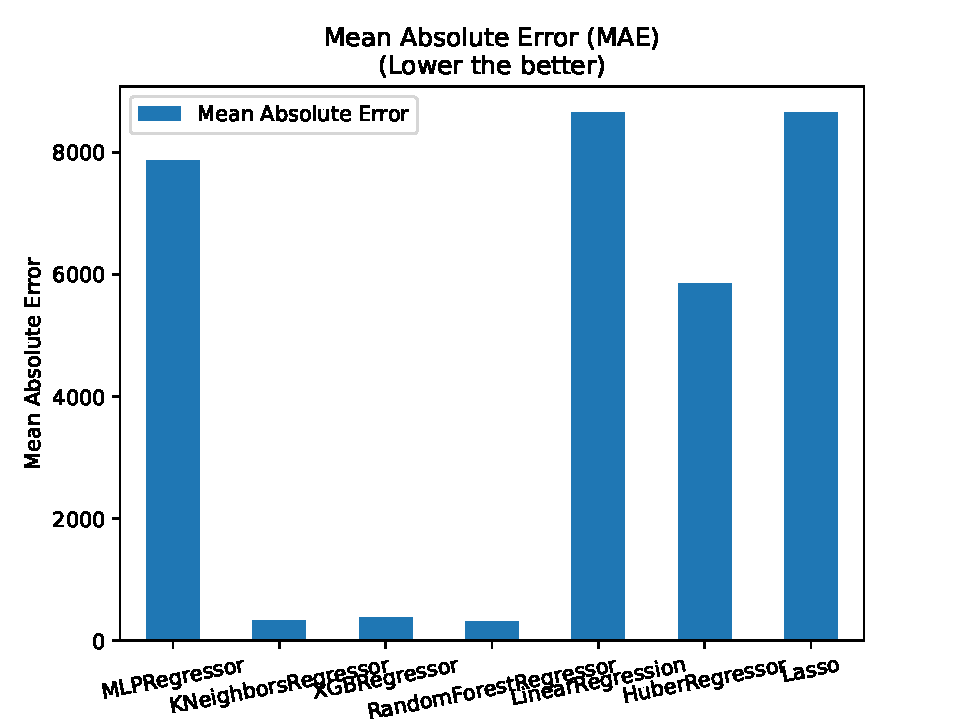
\includegraphics[width=\textwidth]{../regression_model/plots/Comparison/Mean_Absolute_Error.pdf}
        \caption{All regressor model mean absolute error results (lower the better)}
        \label{Fig: all_MAE}
    \end{subfigure}
    \hfill
    \begin{subfigure}[b]{0.49\textwidth}
        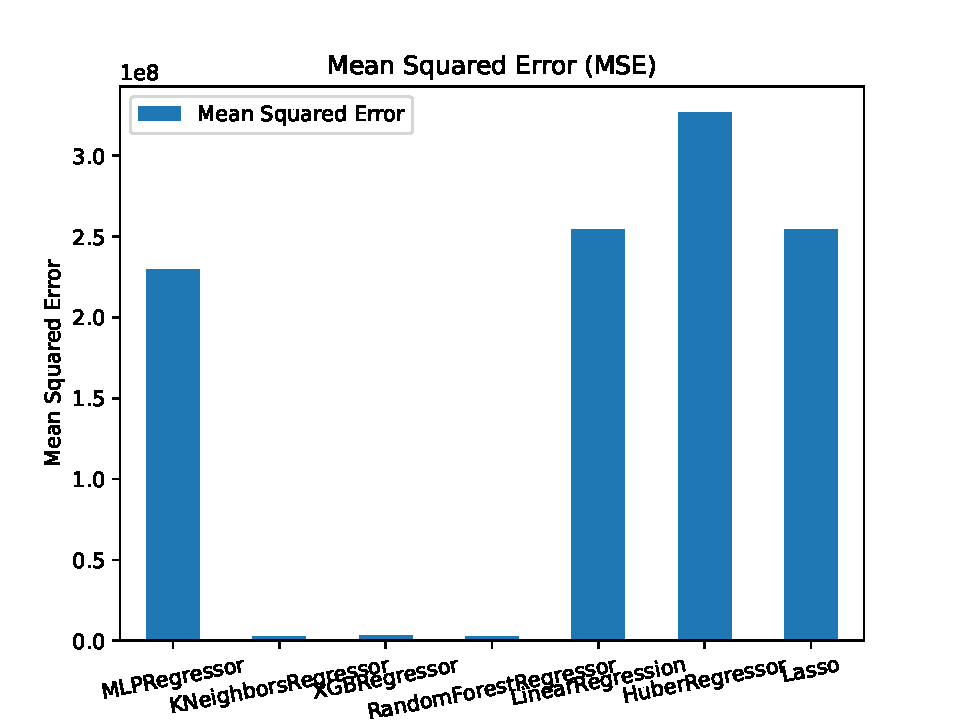
\includegraphics[width=\textwidth]{../regression_model/plots/Comparison/Mean_Squared_Error.pdf}
        \caption{All regressor model squared absolute error results (lower the better)}
        \label{Fig: all_MSAE}
    \end{subfigure}
    \vskip\baselineskip
    \begin{subfigure}[b]{0.49\textwidth}
        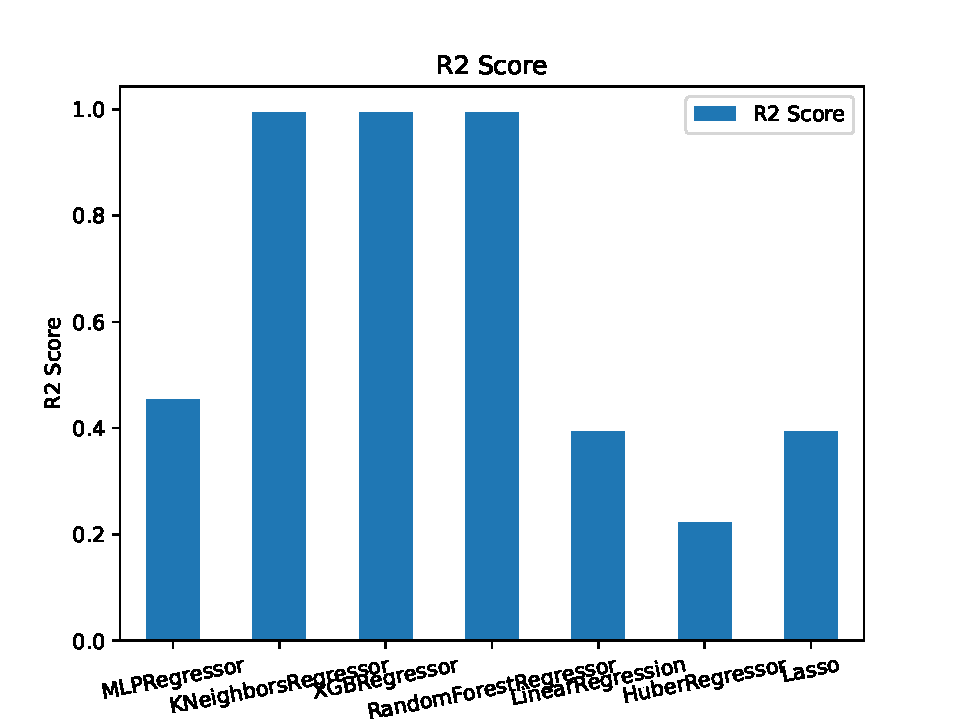
\includegraphics[width=\textwidth]{../regression_model/plots/Comparison/R2_Score.pdf}
        \caption{All regressor model $R^2$ results}
        \label{Fig: all_R2}
    \end{subfigure}
    \hfill
    \begin{subfigure}[b]{0.49\textwidth}
        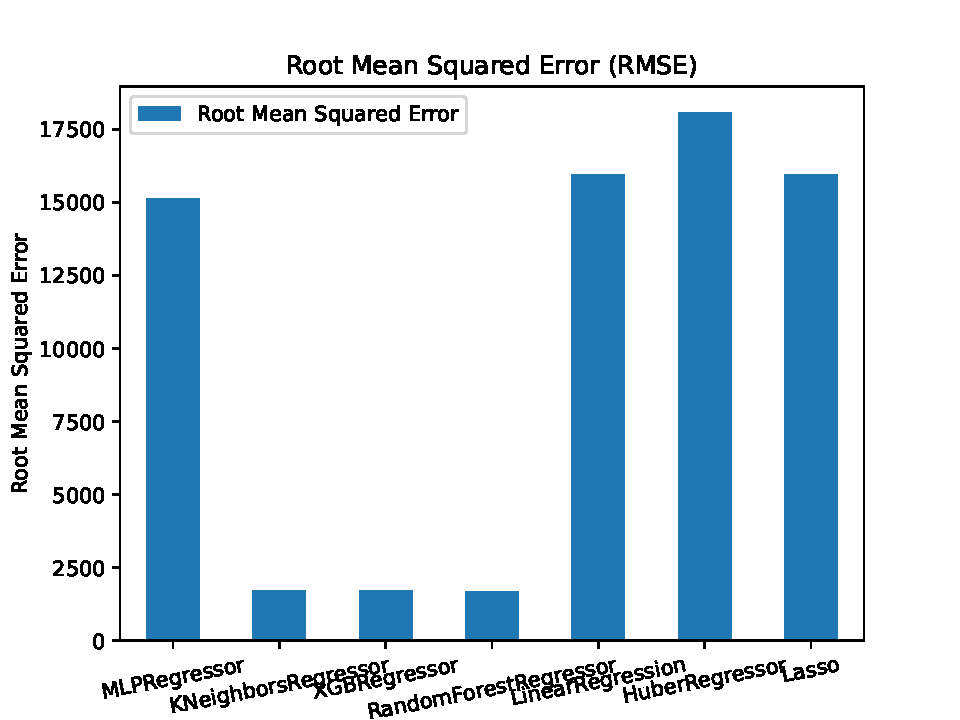
\includegraphics[width=\textwidth]{../regression_model/plots/Comparison/Root_Mean_Squared_Error.pdf}
        \caption{All regressor model root mean squared error results (lower the better)}
        \label{Fig: all_RMSE}
    \end{subfigure}
\end{figure}

% \begin{figure}
%     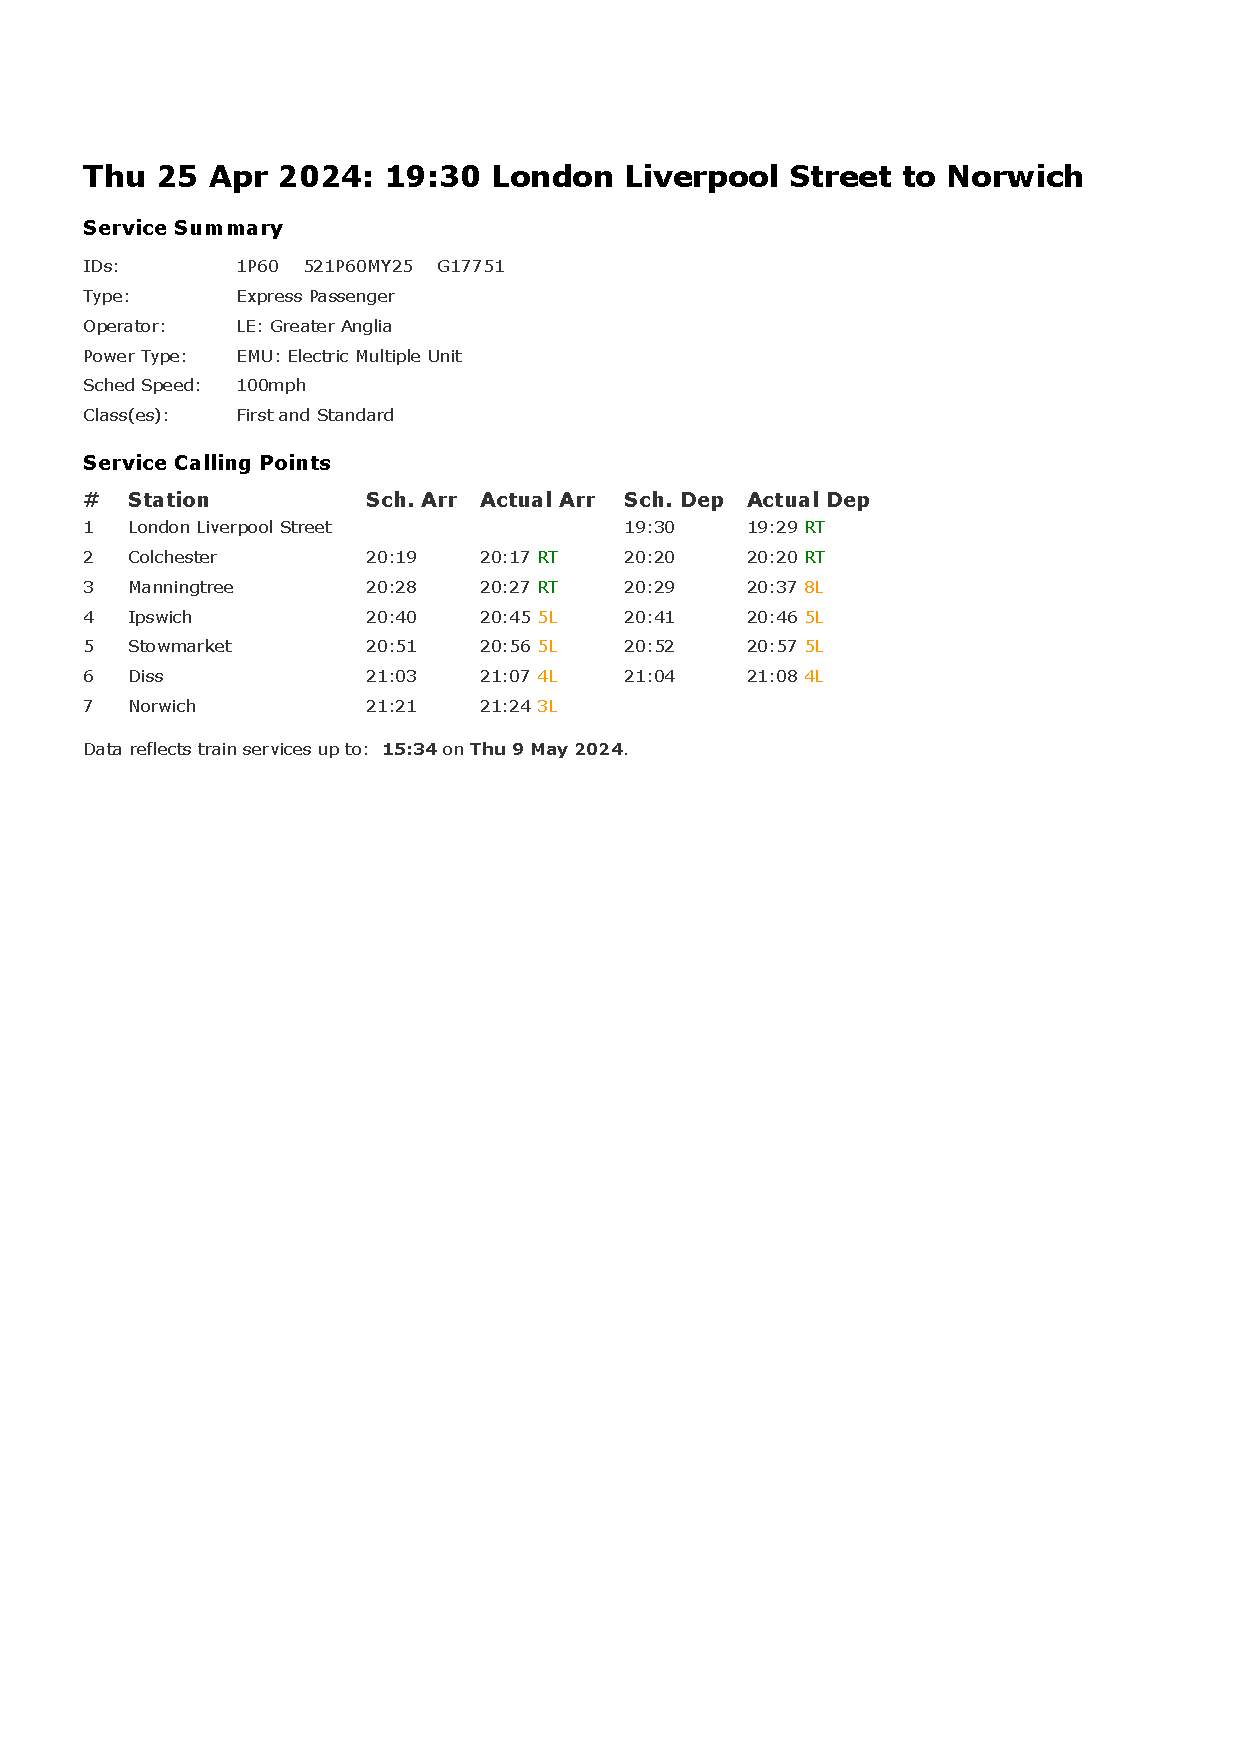
\includegraphics{Diagrams/Exmple of train times/Late/Service Information_25-04-24.pdf}
%     \caption[short]{An eaxmple of a real train journey}
% \end{figure}

\begin{figure}[!htbp]
    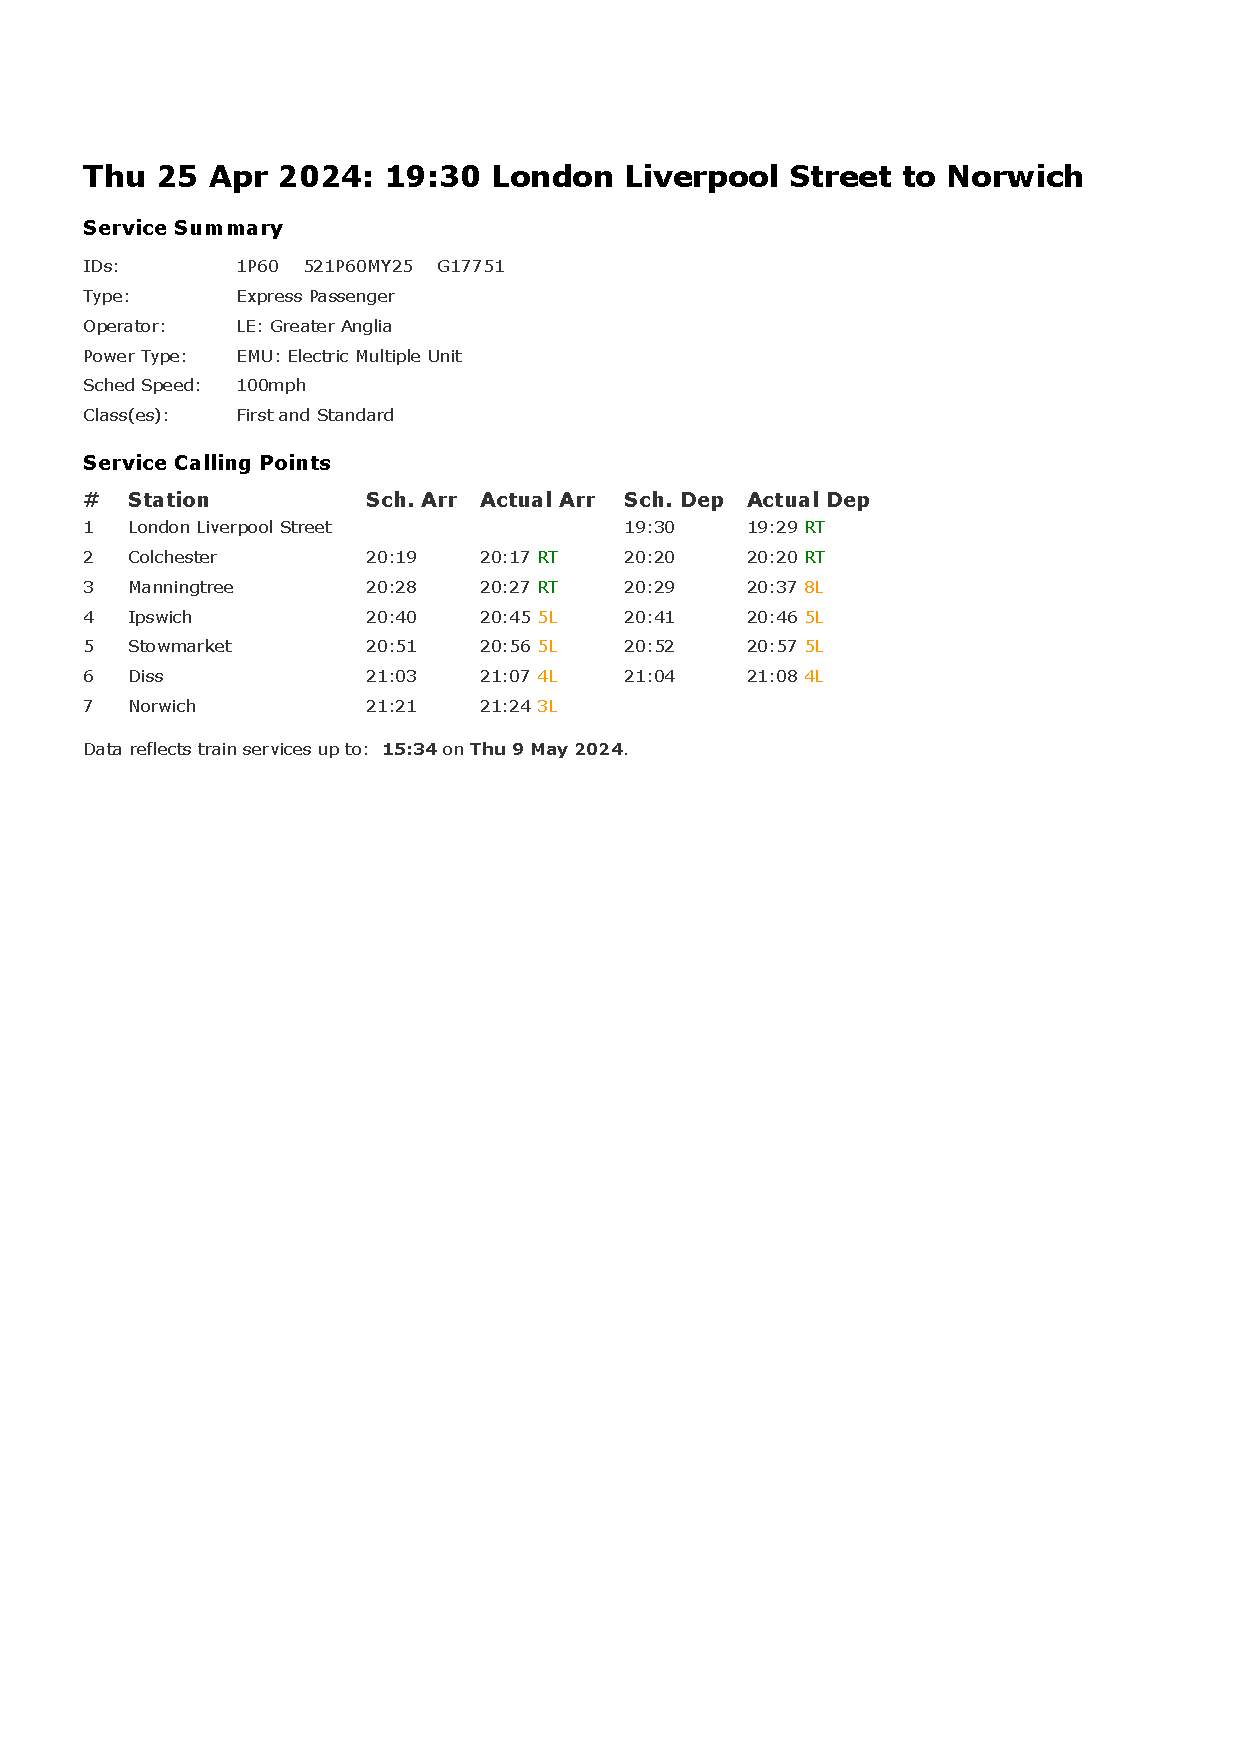
\includegraphics[trim=0 480 0 0]{Diagrams/Exmple of train times/Late/Service Information_25-04-24.pdf}
    \caption[short]{An example of a delayed train journey}
    \label{fig: real delayed train times}
\end{figure}

\begin{figure}[!htbp]
    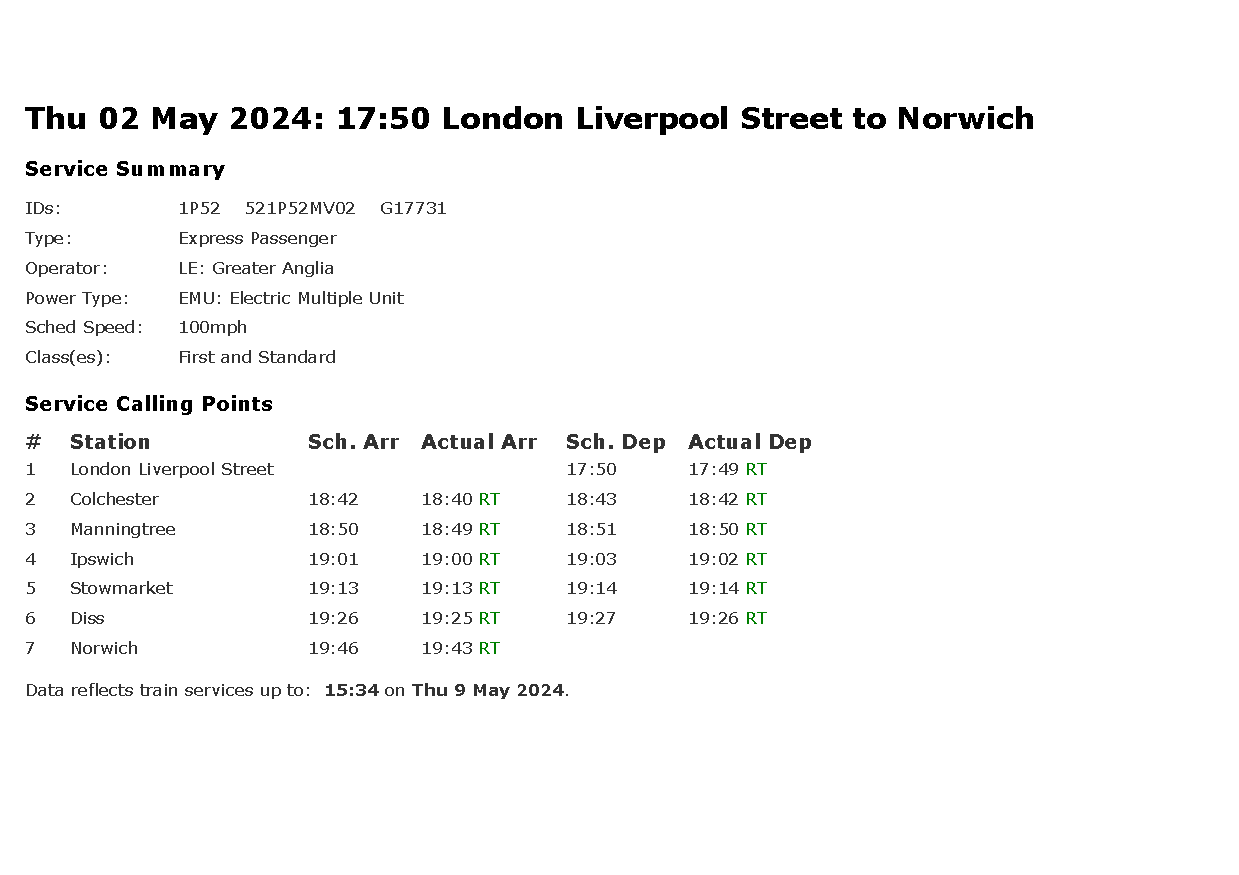
\includegraphics[trim=0 80 0 0]{Diagrams/Exmple of train times/On-Time/Service Information_02-05-24.pdf}
    \caption[short]{An example of an on-time train journey}
    \label{fig: real on-time train times}
\end{figure}

\begin{figure}[!htbp]
    \centering
    \begin{subfigure}[b]{\textwidth}
        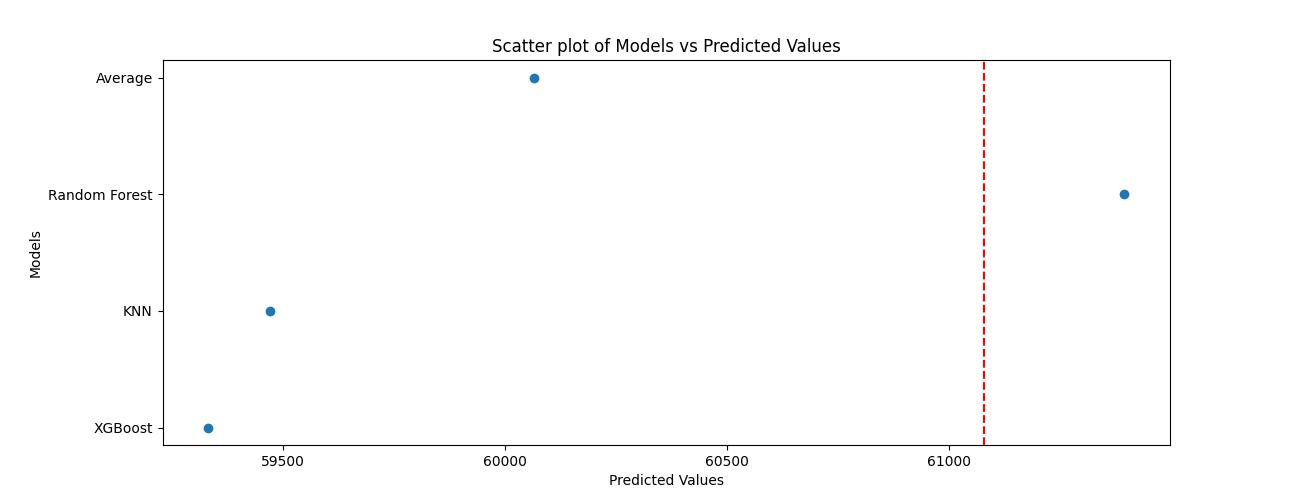
\includegraphics[width=\textwidth]{../regression_model/plots/Comparison/Scatter plot of Models vs Predicted Value 61080.jpeg}
        \caption[short]{}
        \label{}
    \end{subfigure}
    \par
    \begin{subfigure}[b]{\textwidth}
        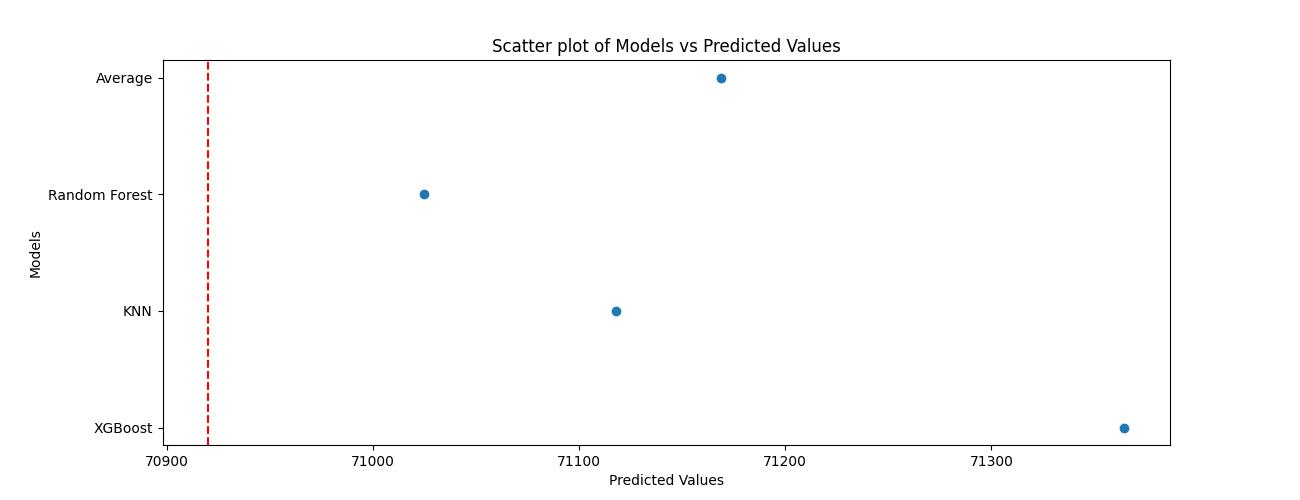
\includegraphics[width=\textwidth]{../regression_model/plots/Comparison/Scatter plot of Models vs Predicted Value 70920.jpeg}
        \caption[short]{}
        \label{}
    \end{subfigure}
    \par
    % \vskip\baselineskip
    \begin{subfigure}[b]{\textwidth}
        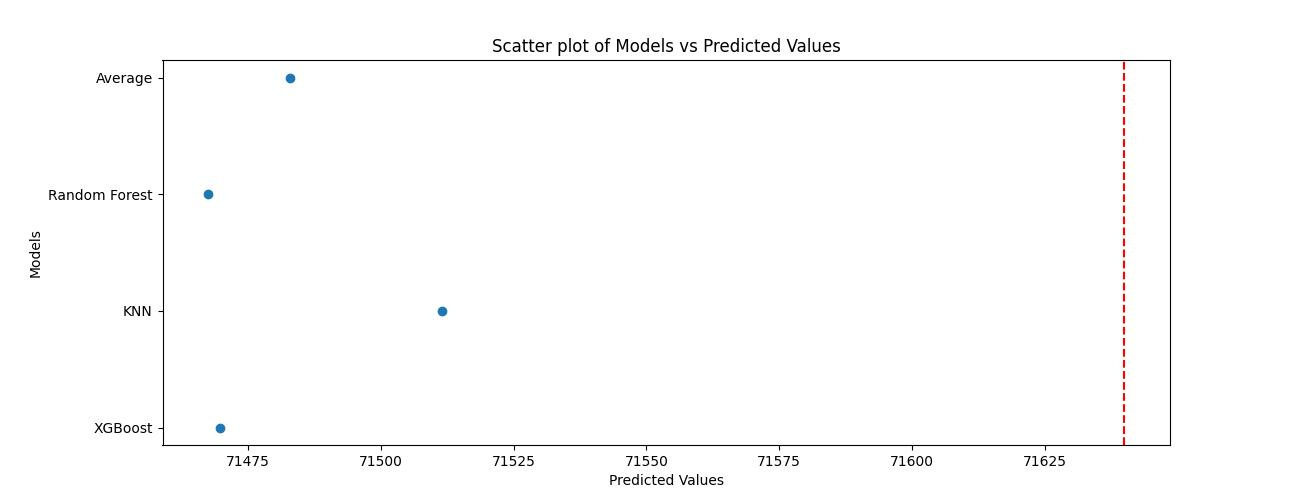
\includegraphics[width=\textwidth]{../regression_model/plots/Comparison/Scatter plot of Models vs Predicted Value 71640.jpeg}
        \caption[short]{}
        \label{}
    \end{subfigure}
    \caption[short]{Regression model predicted arrival time at Norwich from London Liverpool Street if delayed at Ipswich. The red dotted vertical line is ground truth.}
    \label{fig: Regression model predicted arrival time at Norwich from London Liverpool Street}
\end{figure}

\begin{figure}[!htbp]
    \centering
    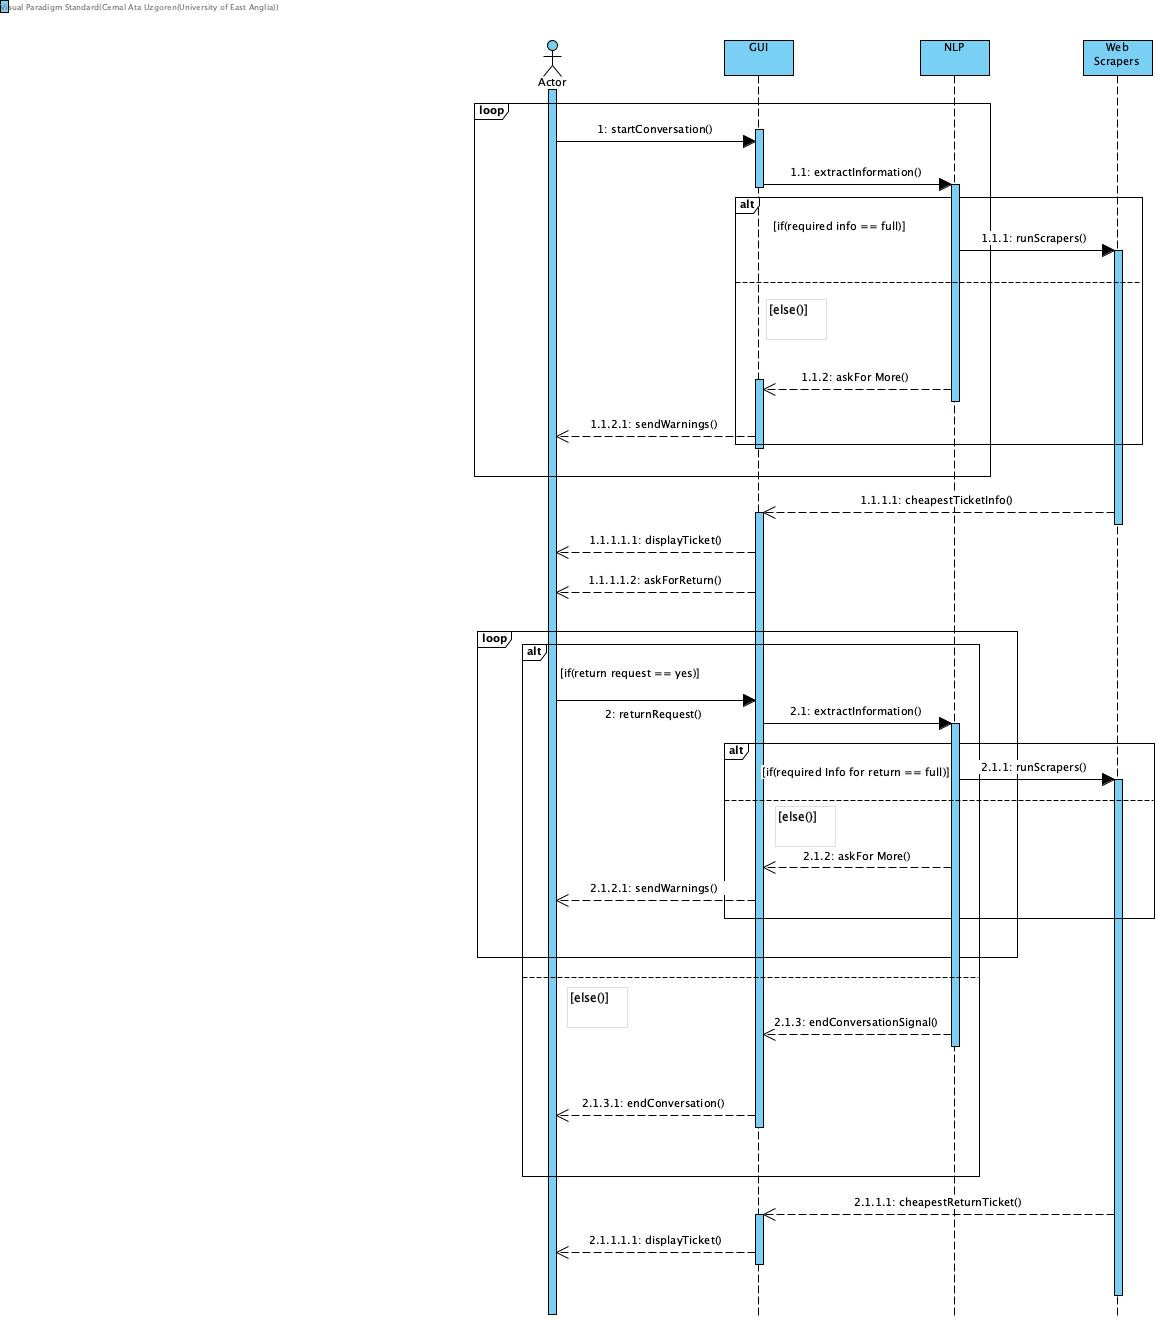
\includegraphics[trim= 350 0 0 0,width= 0.8\textwidth]{Diagrams/ata_diags/Sequence Diagram of Part-1.jpg}
    \caption{A sequence diagram for the chatbot's ticket scraping mechanism}
    \label{Fig: seq diag ticket scraping}
\end{figure}

\begin{figure}[!htbp]
    \centering
    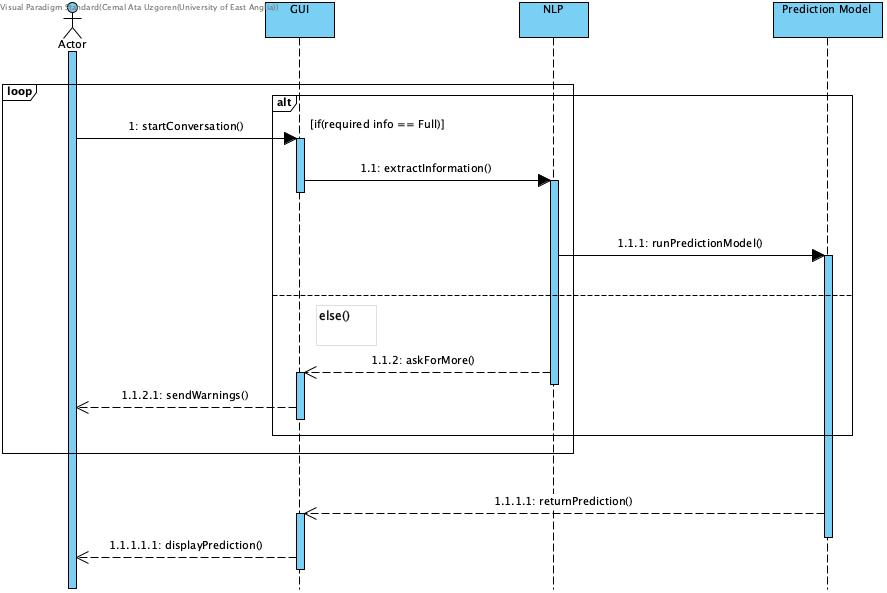
\includegraphics[width= 0.8\textwidth]{Diagrams/ata_diags/Sequence Diagram of Part-2.jpg}
    \caption{A sequence diagram for the chatbot's delayed journey mechanism}
    \label{Fig: seq diag delay prediction}
\end{figure}

\begin{figure}[!htbp]
    \centering
    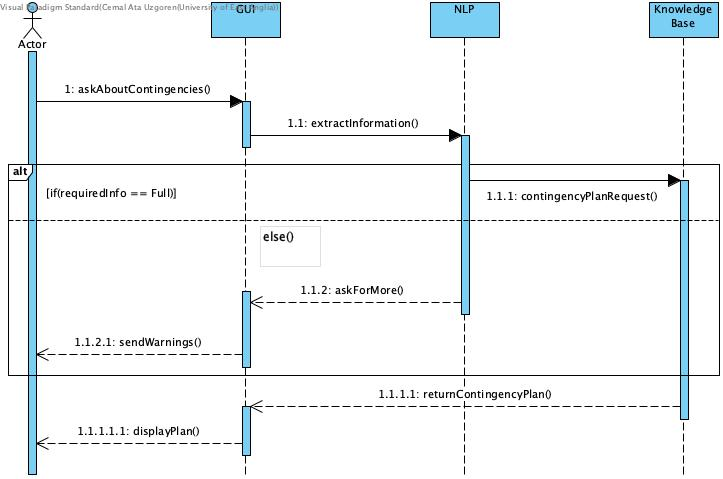
\includegraphics[width= 0.8\textwidth]{Diagrams/ata_diags/Sequence Diagram for Part-3.jpg}
    \caption{A sequence diagram for the chatbot's contingency mechanism}
    \label{Fig: seq diag contingency}
\end{figure}

\begin{figure}[!htbp]
    \centering
    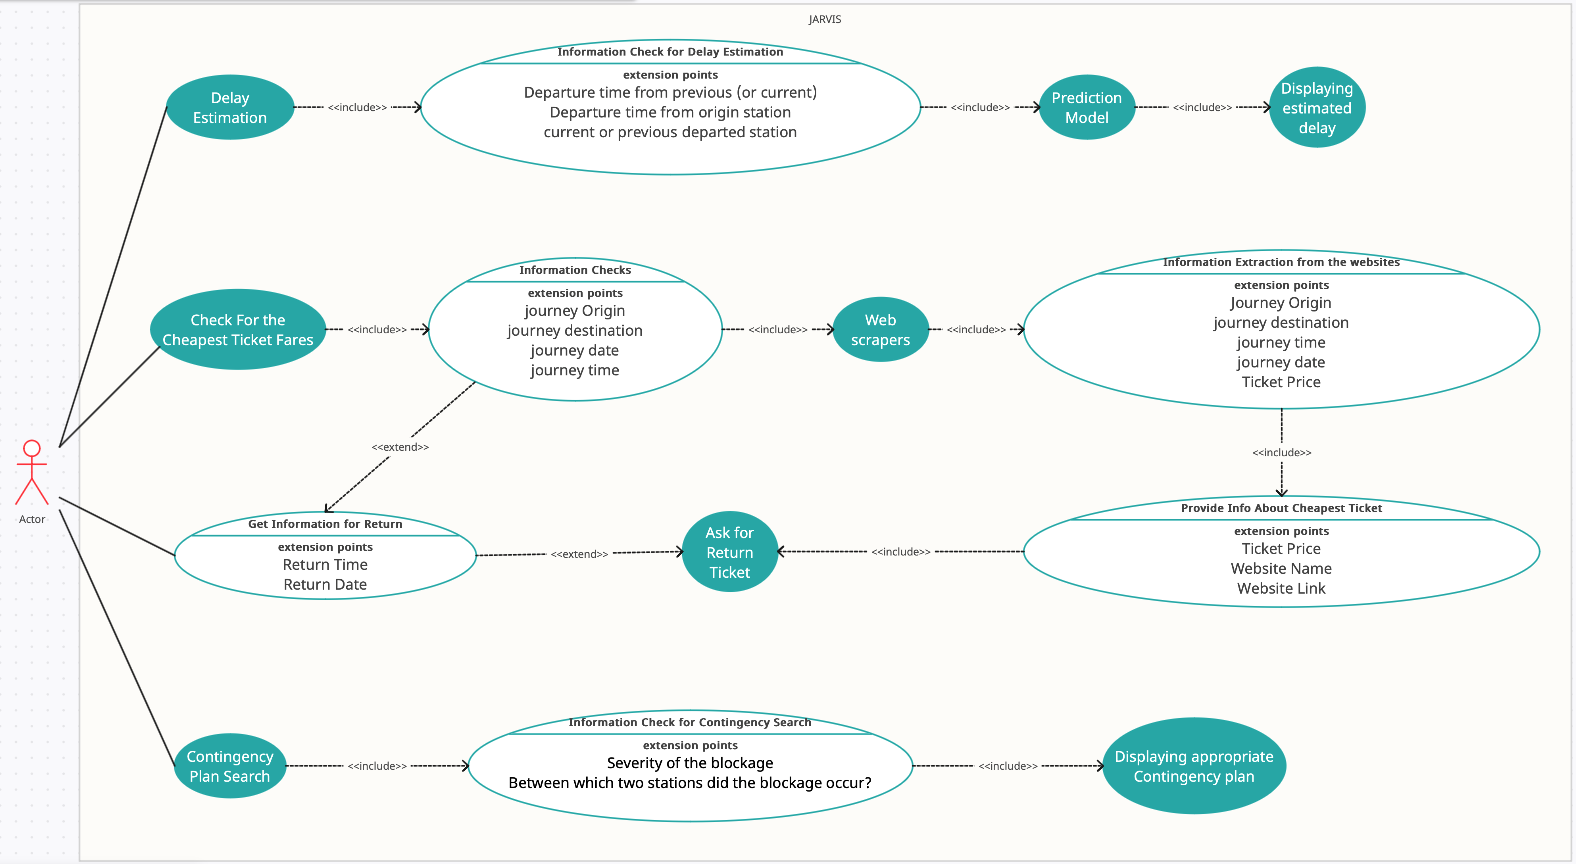
\includegraphics[width=\textwidth]{Diagrams/ata_diags/image.png}
    \caption{A use case diagram for the entire chatbot system}
    \label{Fig: use case whole system}
\end{figure}

\begin{figure}[!htbp]
    \centering
    % 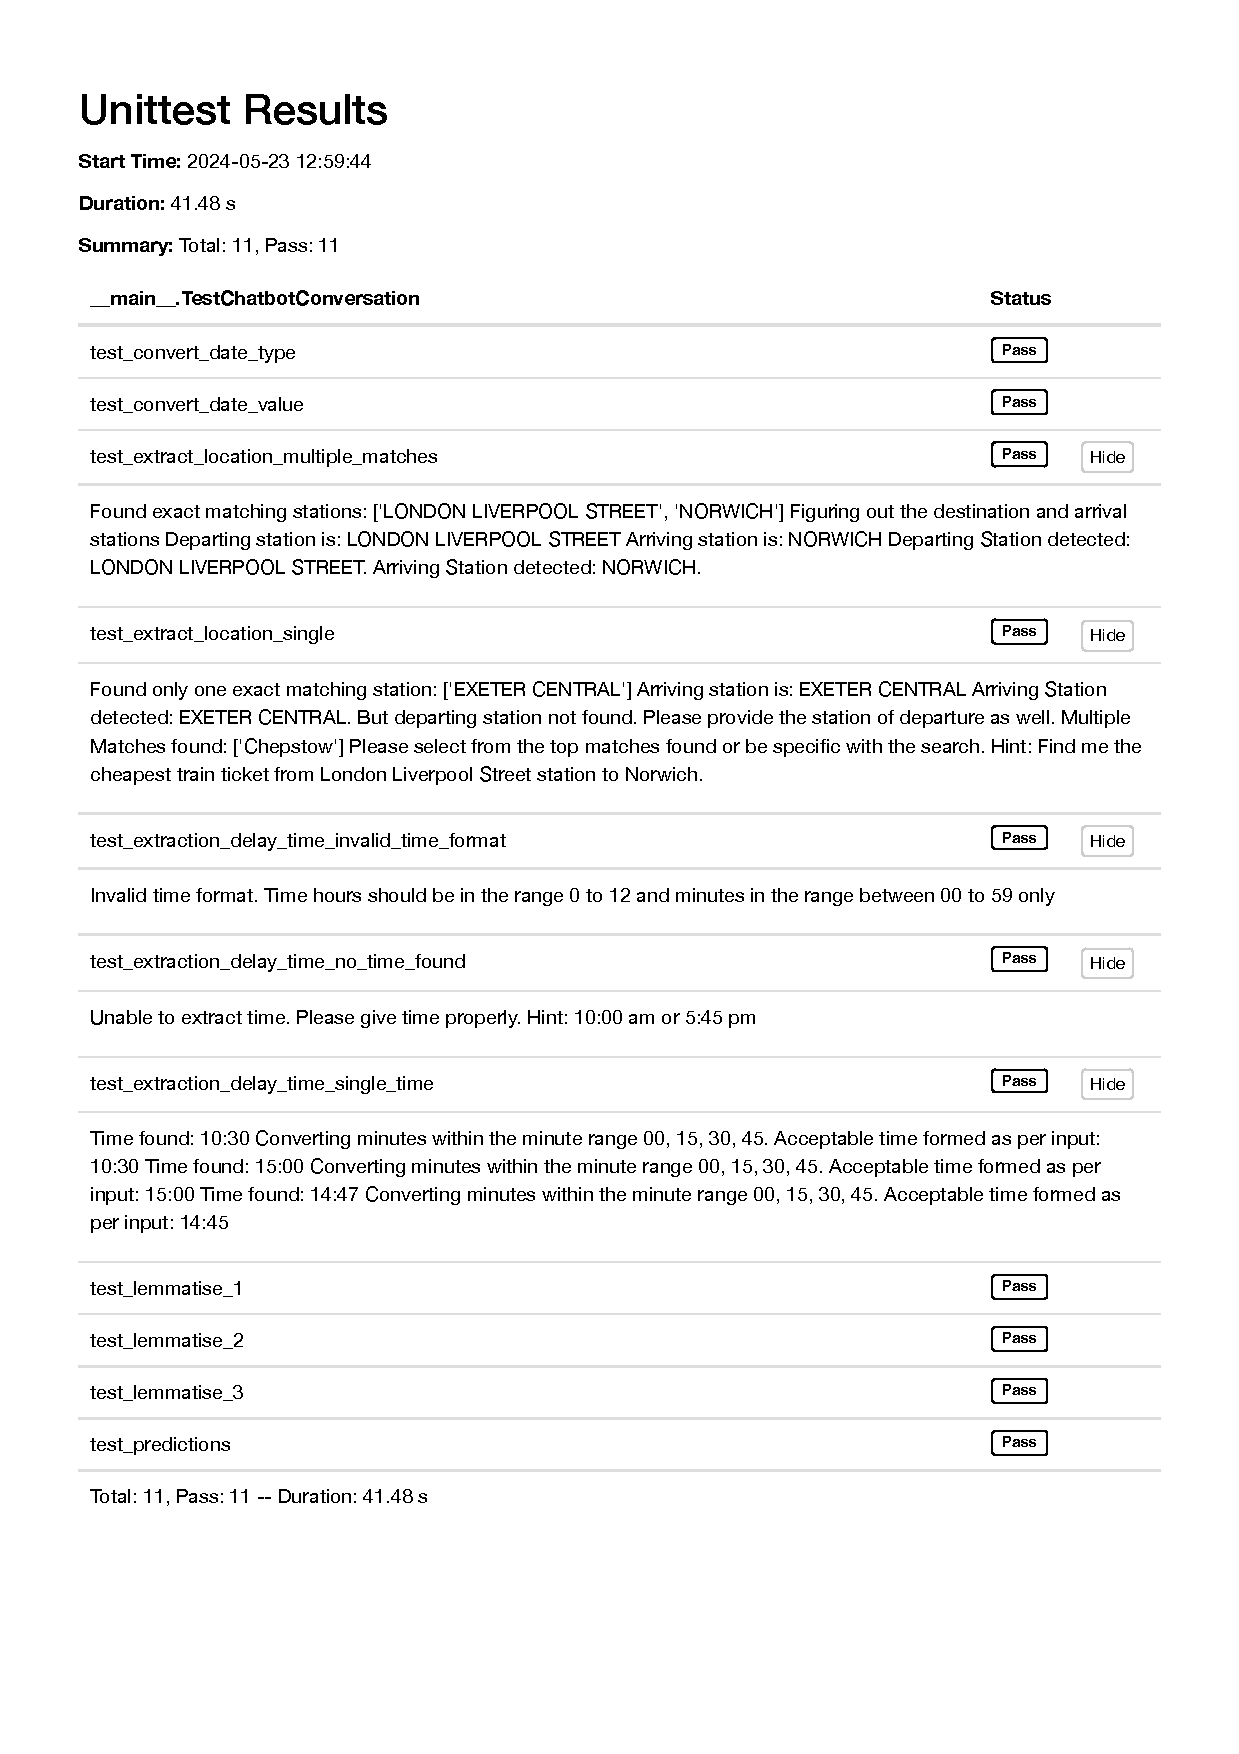
\includegraphics[trim = 0 100 0 0, width=\textwidth]{Diagrams/Unit_Test_HTML/Unittest Results.pdf}
    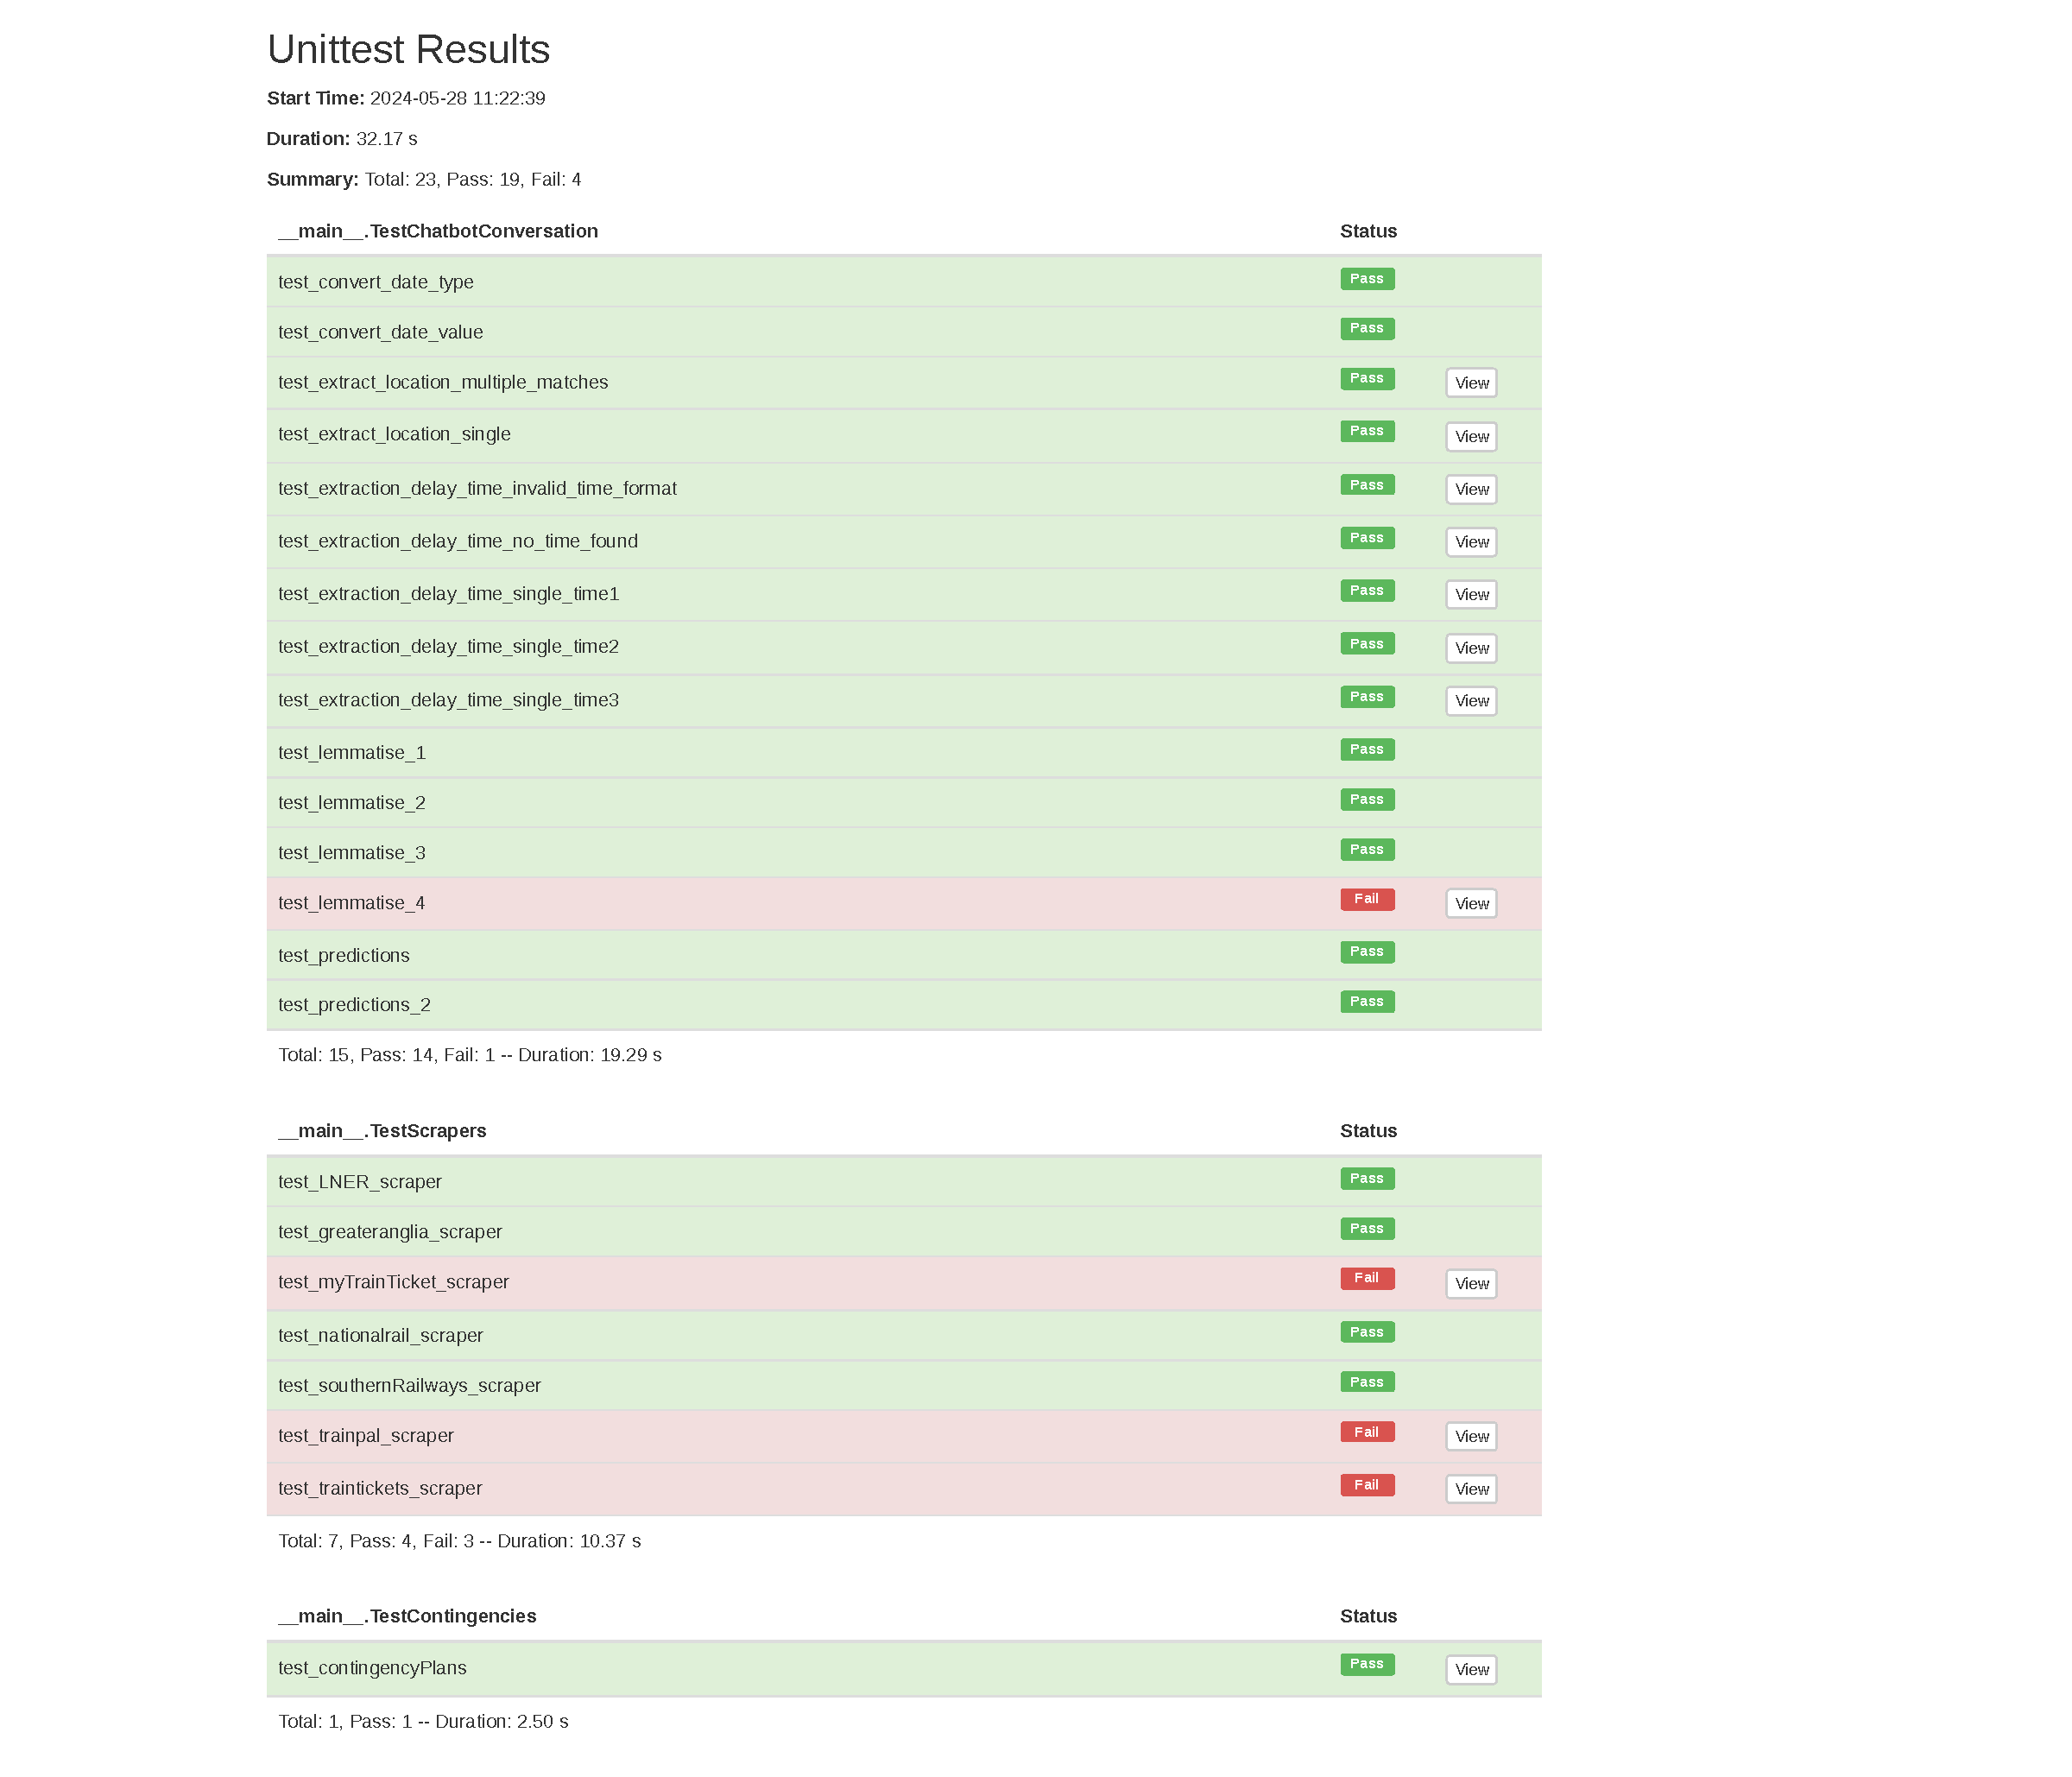
\includegraphics[width=1.2\textwidth]{../Tests/TestResults_TestChatbotConversation_TestScrapers_TestContingencies_2024-05-28_11-22-39.pdf}
    \caption{Results from the unit tests executed during the development of the chatbot}
    \label{Fig: unit test results}
\end{figure}

\clearpage
\subsection{Group Work}
\begin{table}[H]
    \centering
    \begin{tabular}{|l|c|}
        \hline
        \textbf{Team Member} & \textbf{Contribution (\%)} \\
        \hline
        Cemal Ata Uzgoren & 33.33\% \\
        \hline
        Aman Seth & 33.33\% \\
        \hline
        Joshua Newton & 33.33\% \\
        \hline
    \end{tabular}
    \caption{Team Members and their Contributions}
    \label{tab:team_contributions}
\end{table}

\subsubsection{Trello}
Link of the Trello page: \url{https://trello.com/b/CipZLfxi/cmp-7028b-assignment-02}

\begin{figure}[!htbp]
    \centering
    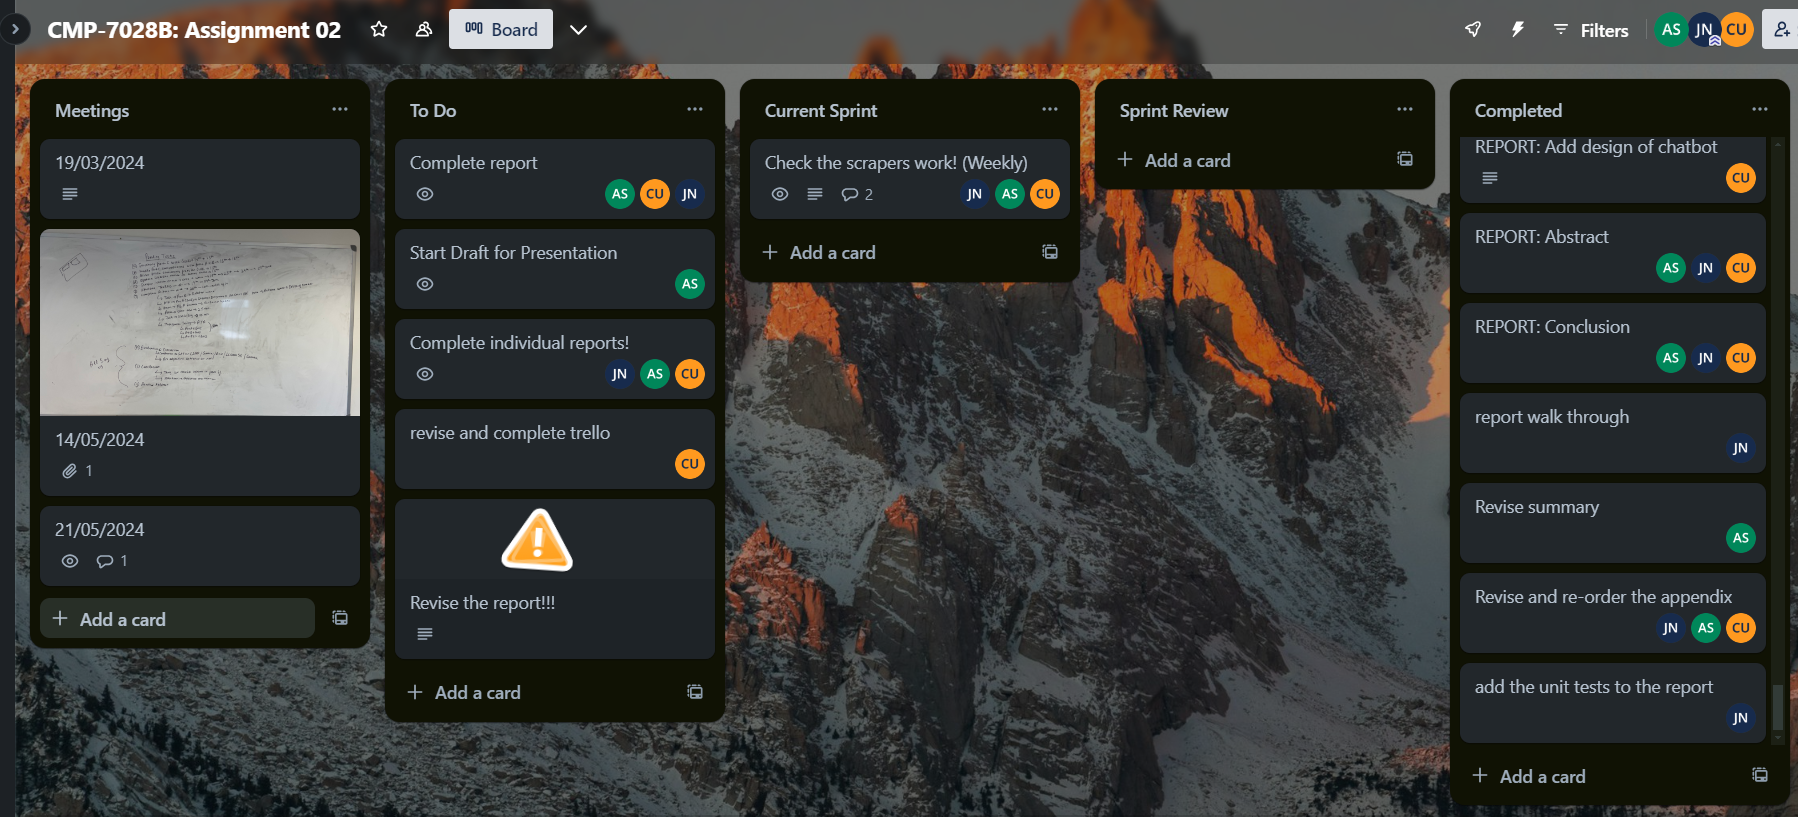
\includegraphics[width=1\linewidth]{Diagrams/Group_work/trello_board.png}
    \caption{Trello Board}
    \label{Fig: trello_ss}
\end{figure}

\begin{figure}[!htbp]
    \centering
    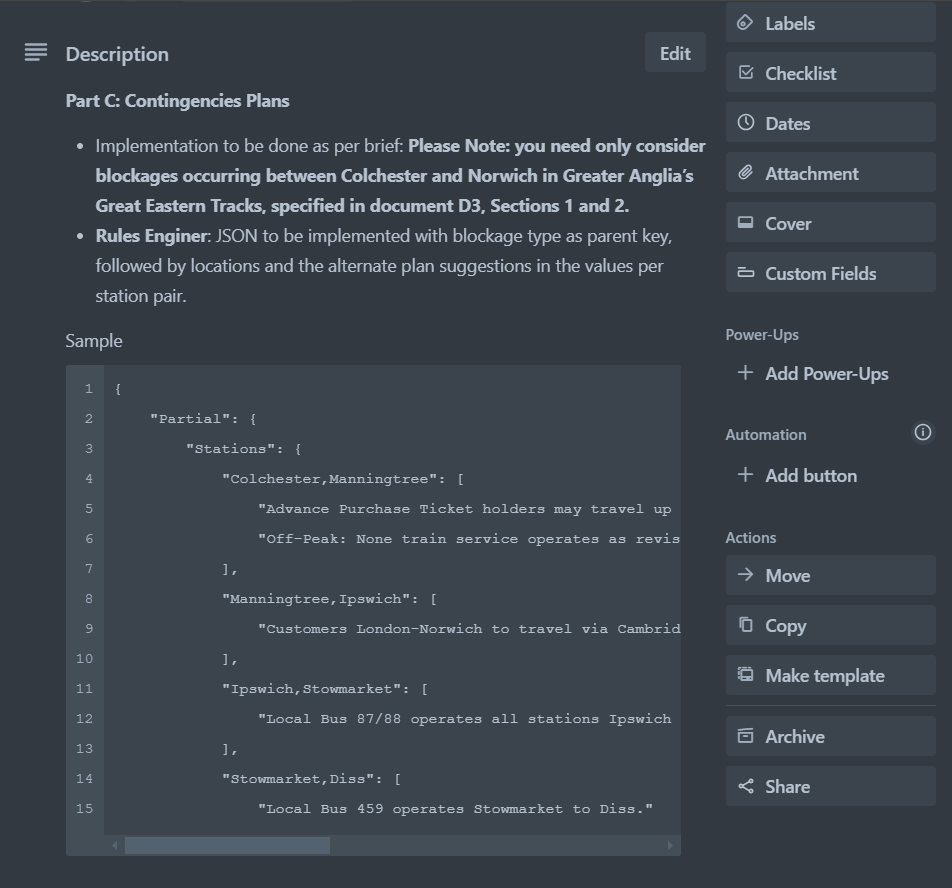
\includegraphics[width=1\linewidth]{Diagrams/Group_work/trello_card.png}
    \caption{Trello Card - Part C}
    \label{Fig: trello_card_c}
\end{figure}

\begin{figure}[!htbp]
    \centering
    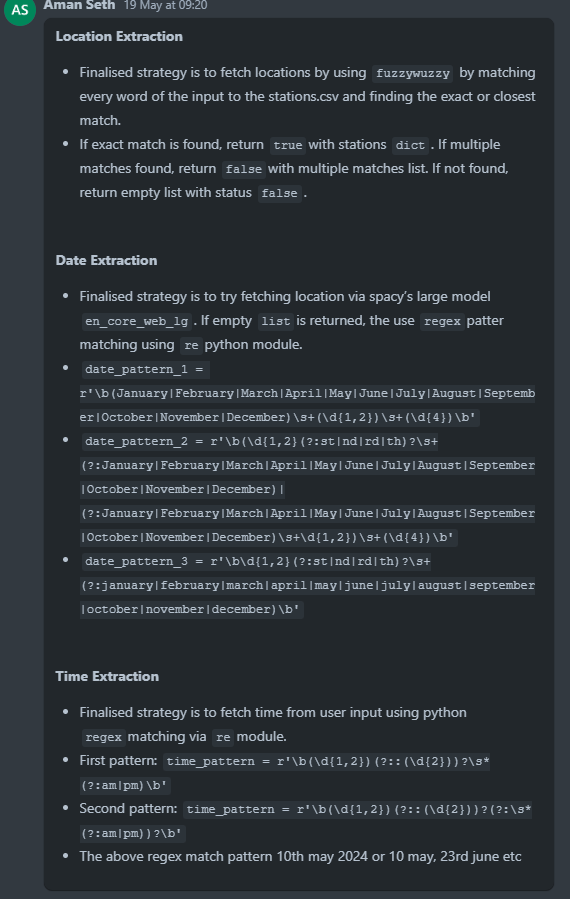
\includegraphics[width=0.8\textwidth]{Diagrams/Group_work/trello_card_2.png}
    \caption{Trello Card - Name Entity Recognition}
    \label{Fig: trello_card_nlp}
\end{figure}

\clearpage
\subsubsection{Github}
Link of the Github page : \url{https://github.com/Staying-Inside/chatbot.git}

\begin{figure}[!htbp]
    \centering
    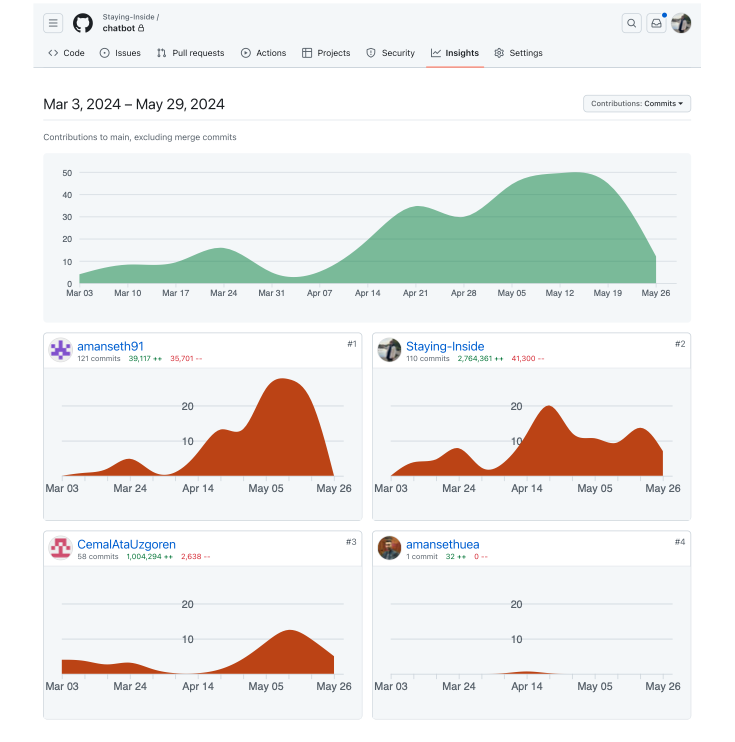
\includegraphics[width=1\linewidth]{Diagrams/Group_work/Github_insights.png}
    \caption{Insights of the project repository}
    \label{fig:insights_github}
\end{figure}

\clearpage

\begin{figure}[!htbp]
    \centering
    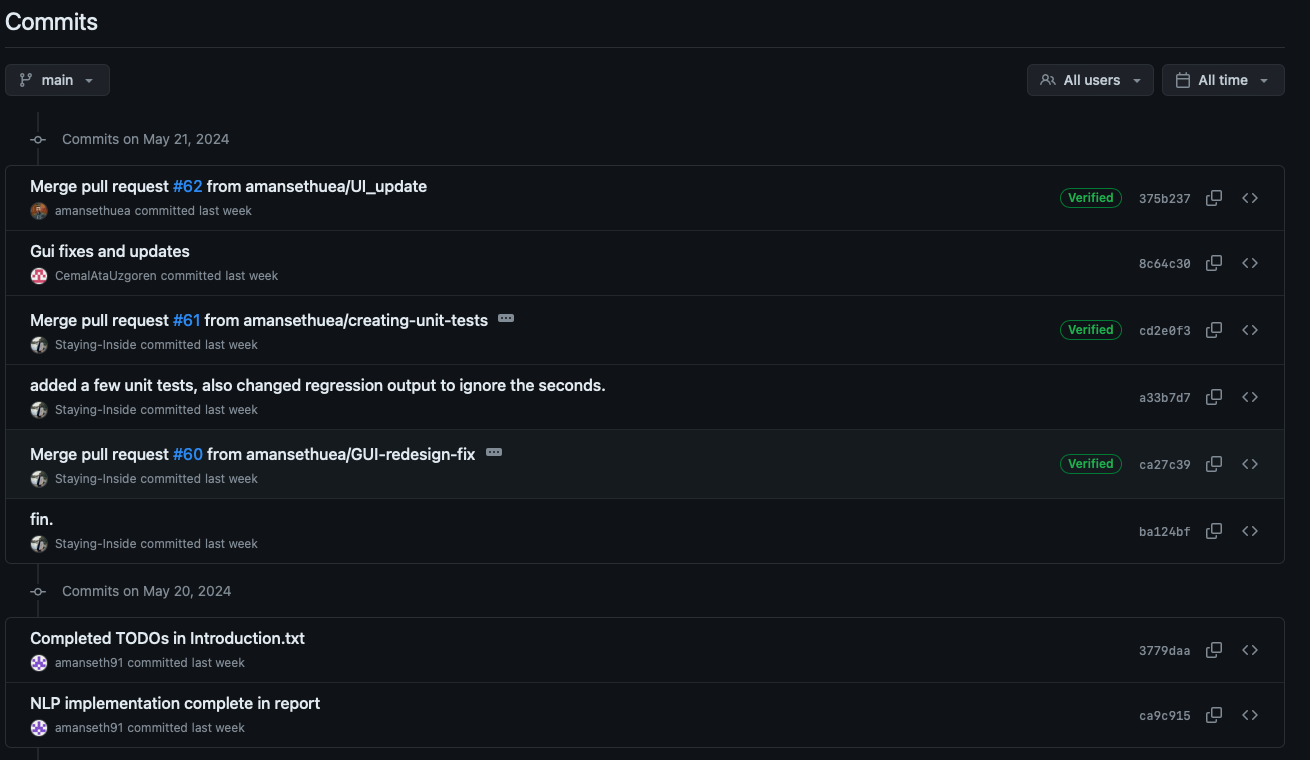
\includegraphics[width=1\linewidth]{Diagrams/Group_work/Github_commit_page.png}
    \caption{Commit screen of the project repository}
    \label{fig:commit_github}
\end{figure}

\clearpage

\subsubsection{Design phase}
\begin{figure}[!htbp]
    \centering
    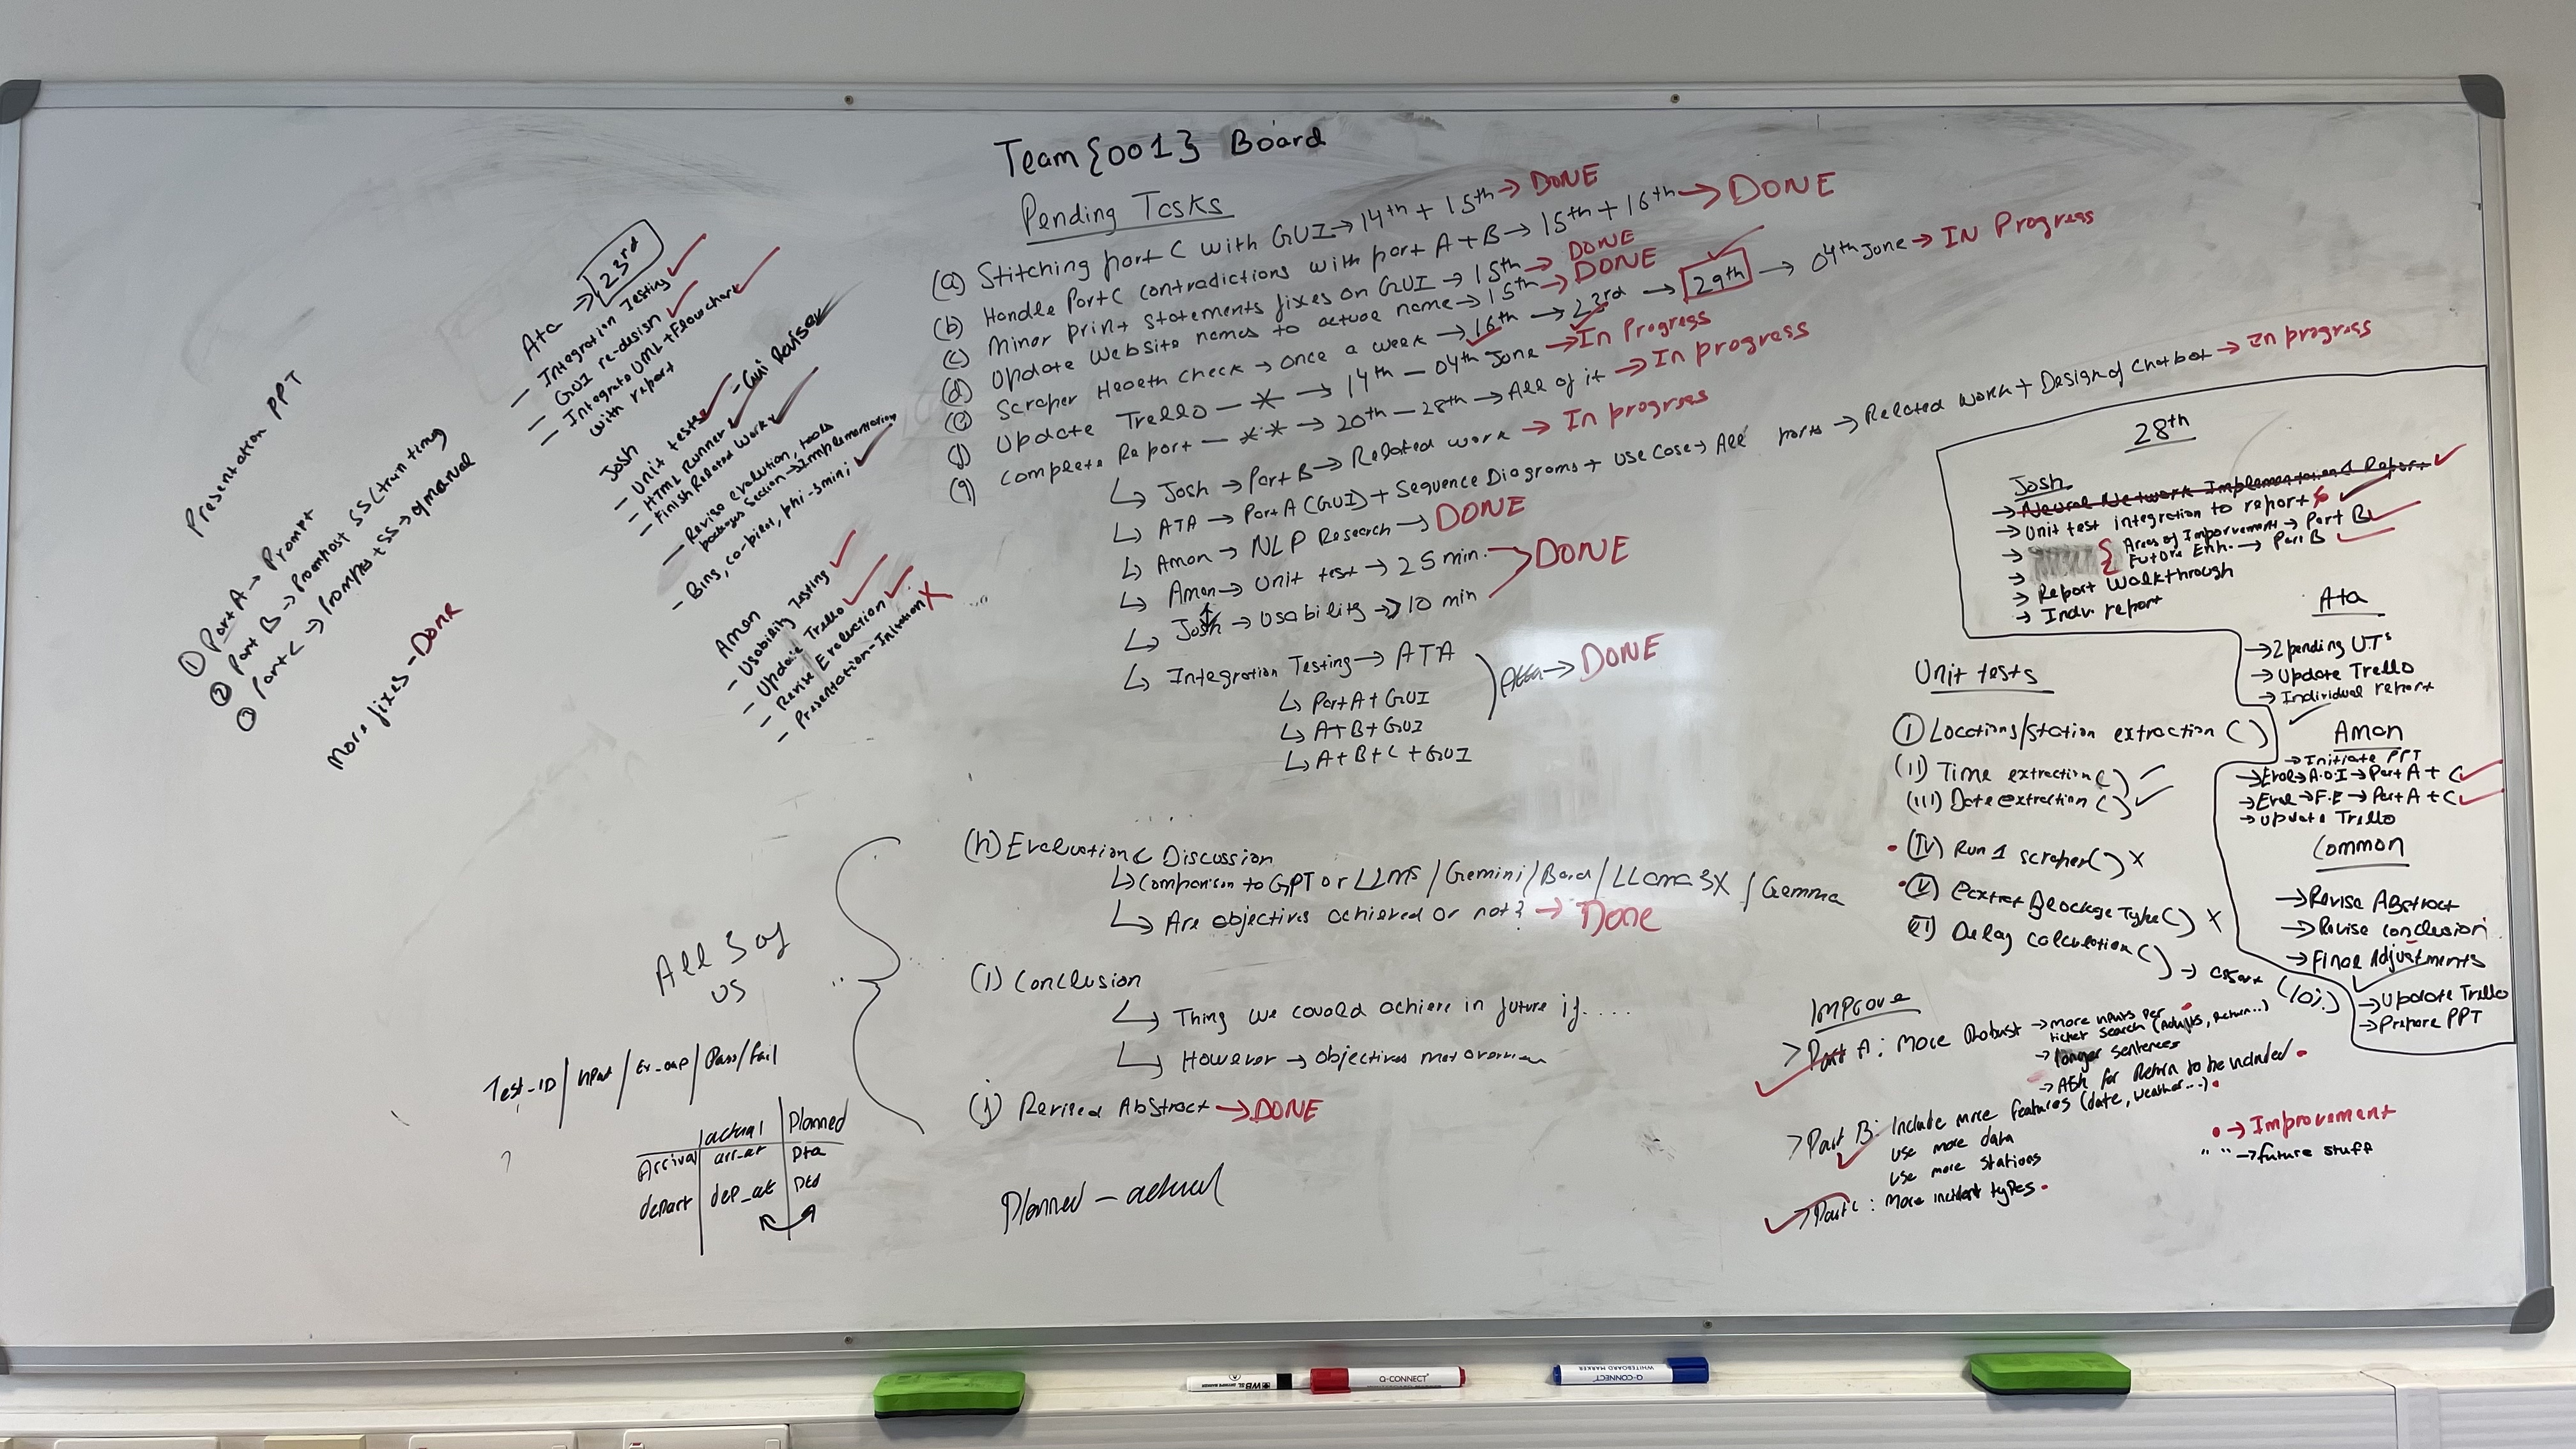
\includegraphics[width=1\linewidth]{Diagrams/Group_work/Group_whiteboard.jpg}
    \caption{Work-load distribution for reporting}
    \label{fig:lab2}
\end{figure}

\begin{figure} [!htbp]
    \centering
    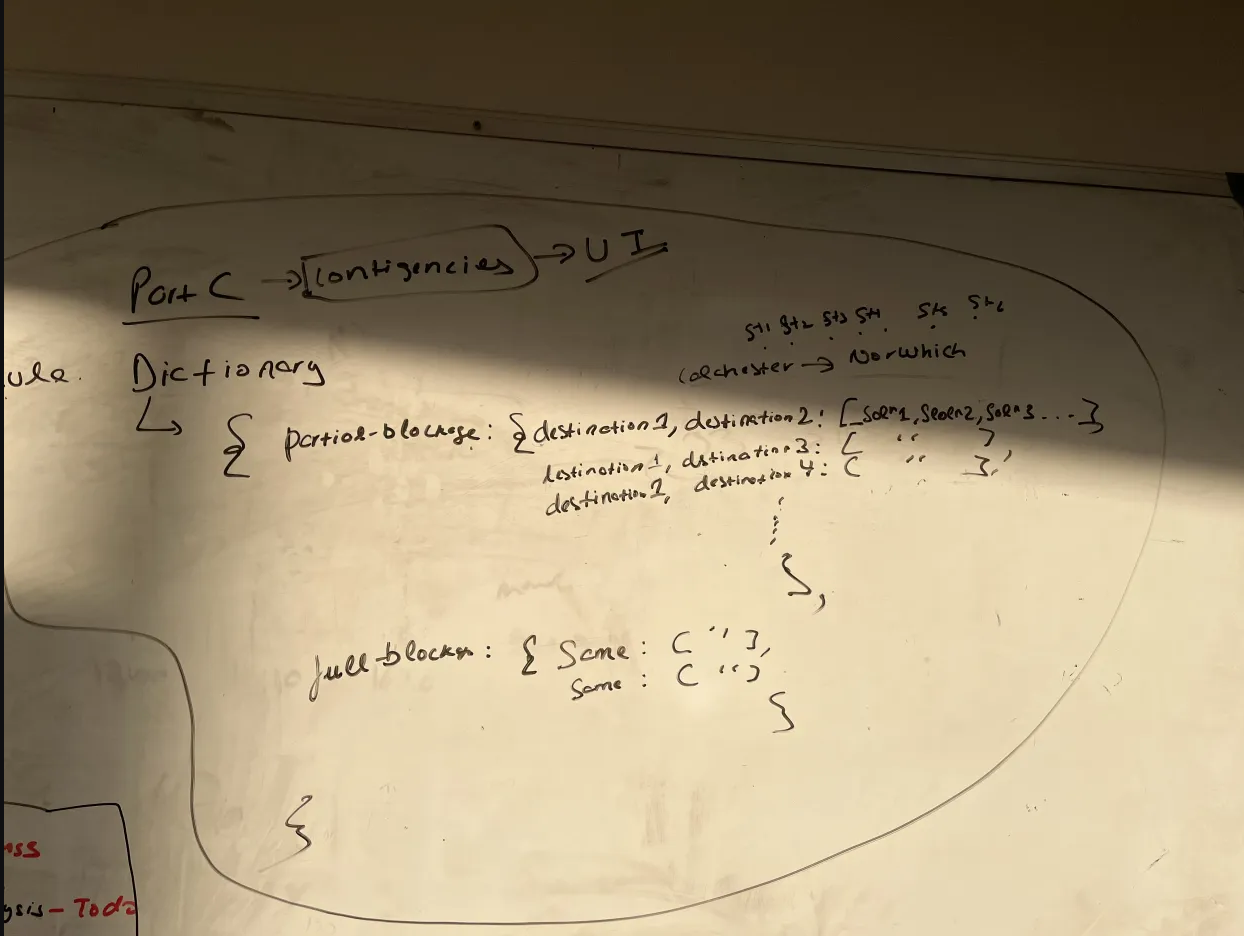
\includegraphics[width=1\linewidth]{Diagrams/Group_work/lab_Handwritings.png}
    \caption{Part-3 plan}
    \label{fig:lab1}
\end{figure}

\clearpage
\subsubsection{Coding Phase}
\textbf{Spawning Python via JS (GUI)}
\begin{figure} [!htbp]
    \centering
    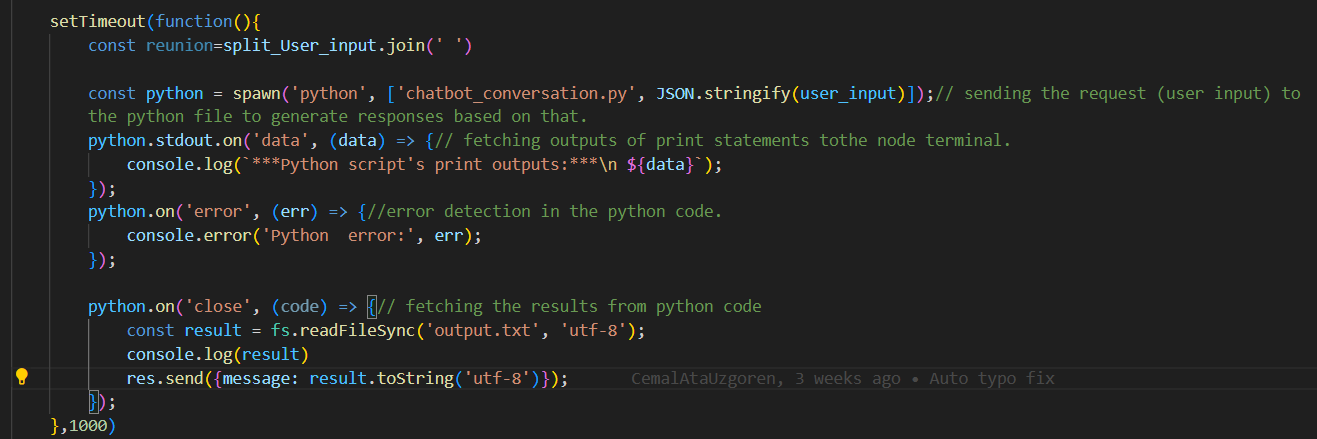
\includegraphics[width=1\linewidth]{Diagrams/Group_work/spawn.png}
    \caption{Code: Spawning Python NLP code via JS}
    \label{fig:python_spawn}
\end{figure}

\textbf{NLP - Date Extraction}
\begin{figure} [!htbp]
    \centering
    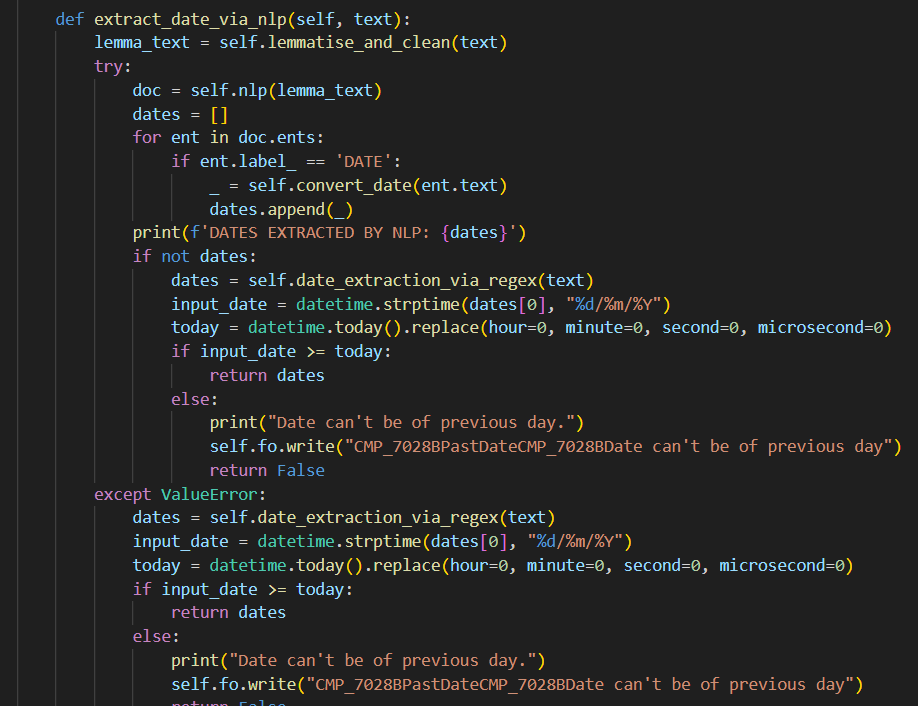
\includegraphics[width=1\linewidth]{Diagrams/Group_work/date_extraction_nlp.png}
    \caption{Code: Date Extraction Mechanism}
    \label{fig:date_extraction_nlp}
\end{figure}

\textbf{Prediction Model}
\begin{figure} [!htbp]
    \centering
    \includegraphics[width=1\linewidth]{Diagrams/Group_work/model_loading_code.png}
    \caption{Code: Model Prediction for Part B}
    \label{fig:model_prediction}
\end{figure}

\textbf{Blockage Type Extraction}
\begin{figure} [!htbp]
    \centering
    \includegraphics[width=1\linewidth]{Diagrams/Group_work/part_c.png}
    \caption{Code: Blockage Type Extraction in Part C}
    \label{fig:part_c_blockage}
\end{figure}

\clearpage
\subsubsection{Testing Phase}
\textbf{Testing Scenario: Part A and B integrity constraint}
The below tests demonstrate that the user cannot directly switch conversation to part B (Delay prediction) if there is an on-going conversation regarding part A (Cheapest train fare search) in place. The user may or may not reset the search explicitly in order to proceed.
\begin{figure} [!htbp]
    \centering
    \includegraphics[width=1\linewidth]{Diagrams/Group_work/testing_1.png}
    \caption{Test: Part A and B Integrity Constraint Check}
    \label{fig:test_1}
\end{figure}

\clearpage
\textbf{Testing Scenario: Part B and A integrity constraint}
The below tests demonstrate that the user cannot directly switch conversation to part A (Cheapest train fare search) if there is an on-going conversation regarding part B (Delay prediction) in place. The user may or may not reset the search explicitly in order to proceed.
\begin{figure} [!htbp]
    \centering
    \includegraphics[width=1\linewidth]{Diagrams/Group_work/testing_2.png}
    \caption{Test: Part B and A Integrity Constraint Check}
    \label{fig:test_2}
\end{figure}